% Created 2021-08-30 Mon 11:33
% Intended LaTeX compiler: pdflatex
\documentclass[11pt]{article}
\usepackage[utf8]{inputenc}
\usepackage[T1]{fontenc}
\usepackage{graphicx}
\usepackage{grffile}
\usepackage{longtable}
\usepackage{wrapfig}
\usepackage{rotating}
\usepackage[normalem]{ulem}
\usepackage{amsmath}
\usepackage{textcomp}
\usepackage{amssymb}
\usepackage{capt-of}
\usepackage{hyperref}
\usepackage{listingsutf8}
\usepackage{minted}
\usepackage{arxiv}
\author{Marco Hassan}
\date{\today}
\title{}
\hypersetup{
 pdfauthor={Marco Hassan},
 pdftitle={},
 pdfkeywords={},
 pdfsubject={},
 pdfcreator={Emacs 27.2.50 (Org mode 9.4.4)}, 
 pdflang={English}}
\begin{document}

\newtheorem{theorem}{Theorem}
\pagenumbering{roman}%- roman numbering for first few pages
%% \title{Parameter Learning in Bayesian Networks under Uncertain Evidence  \textendash  \ An Exploratory Research.}
%% \author{
%%   Marco Hassan 	           	\\
%%   Zurich, CH		\\
%%   \\
%%   \\n
%%   Master Thesis \\
%%   Presented to the Eidgenossische Teschnische Hochschule Zurich \\
%%   In Fulfillment Of the Requirements for \\ 
%%   the Master of Science in Statistics \\
%%   \\
%%   Supervisor: PhD. Radu Marinescu \\
%%   Co-Supervisor: Dr. Markus Kalisch \\
%%   %% examples of more authors
%%   %% \AND
%%   %% Coauthor \\
%%   %% Affiliation \\
%%   %% Address \\
%%   %% \texttt{email} \\   
%%   %% \And
%%   %% Coauthor \\
%%   %% Affiliation \\
%%   %% Address \\
%%   %% \texttt{email} \\
%%   %% \And
%%   %% Coauthor \\
%%   %% Affiliation \\
%%   %% Address \\
%%   %% \texttt{email} \\
%% }

%%%%%%%%%%%%%%%%%%%%%%%%%%%%%%%%%%%%%%%%%%%%%%%%%%%%%%%%%%
%%% ETH-Style Latex Template vs. Chosen Structure      %%%
%%%%%%%%%%%%%%%%%%%%%%%%%%%%%%%%%%%%%%%%%%%%%%%%%%%%%%%%%%

%% it is too much work to refactor the entire structure of the latex template.
%% I decided just to adapt the citation style and take all fo the rest of the structure as in my usual documentation
%% there is just some minor difference in such a case.

%% For the title take it from the template and paste it in as you did
%% with the declaration of originality
\begin{article}

\includepdf[pages={-}, scale=1]{pdf/title_page.pdf}
\cleardoublepage

%% \maketitle

\newpage

%%%%%%%%%%%%%%%%%%%%%%%%%%%%%%%%%%%%%%%%%%%%%%%%%
%%% Insert here acknowledgements and abstract %%%
%%%%%%%%%%%%%%%%%%%%%%%%%%%%%%%%%%%%%%%%%%%%%%%%%
%% Dedication (optional)
\markright{}
\vspace*{\stretch{1}}
\begin{center}
    $To \ my \ family,  \ my \ beloved \ ones \ and \ my \ dear \ friends$
    \newline
    $that \ make \ difficult \ times \ easier \ to \ face.$
\end{center}
\vspace*{\stretch{2}}

%%%%%%%%%%%%%%%%%%%%%%%%%%%%%%%%%%%%%%%%
%%% Abstract                         %%%
%%%%%%%%%%%%%%%%%%%%%%%%%%%%%%%%%%%%%%%%
 
\newpage
\markboth{Abstract}{Abstract}
\begin{abstract}
  This study deals primarily with the topic of parameter learning in Bayesian Networks.
  In its first sections it proposes a general literature overview of parameter learning
  in the case of Maximum Likelihood Estimation under complete evidence.
  A general introduction to the concept of likelihood decomposability
  is provided before rigorously exposing the EM-algorithm as a viable choice for
  parameter estimation when the decomposability property does not hold and the maximization problem is a nasty multimodal function.
  Given the properties of the EM-algorithm, we will argue that it is possible to generalize the algorithm to
  deal with the case of parameter learning in a full-bayesian learning setting by adjusting the maximization step.
  The second part of study leverages the classic theory exposed in the previous sections to deal with the
  case of parameter learning in the case of uncertain evidence. Augmenting the arguments proposed in \cite{Wasserkrug_all}
  the study will argue that upon finding a constrained joint distribution for the probabilistic graphical model
  that satisfies the constrains imposed by the uncertain evidence, the EM-algorithm might be used for obtaining a
  sensible network parameterization with slight adjustments as the virtual evidence method of \cite{pearl1987evidential}.
  The study shows then by example that that such methods are easily integrable in classical statistical software as
  in the extension of the \href{https://github.com/radum2275/merlin}{merlin}
  engine.
\end{abstract}

% keywords can be removed
\keywords{Graphical Models \and Iterative Methods \and Bayesian Networks \and Bayesian Statistics \and Parameter Learning \and Bayesian Learning \and Uncertain Evidence \and EM-algorithm \and I-projection \and Inference \and Clique Algorithms}

\newpage

\tableofcontents

\newpage

\listoffigures
\listofalgorithms
\listoftables

\newpage

\markboth{Notation}{Notation}
\section*{Notation}
This section introduces some general notation style used in the script.

Sets - i.e. sets of random variables/nodes, edges - are expressed via
the capital italic notation as \(\mathscr{X}\), \(\mathscr{Y}\). We denote
a single realization of the random variables within the set as \(x\),
\(y\) respectively. Finally we denote a set of realizations via the
following italic notation \(\mathcal{X}\), \(\mathcal{Y}\) respectively.

When expressing the probability of a set of realizations, say
\(P(\mathcal{D})\), we intend the likelihood of that set of realizations
under the given probability function.

Random variables themselves are defined via capital letters, while the
lower case of the respective random variables defines domain
realization of the variables.  For instance \(X_i\) represents
a particular random variable while \(x_i\) represents the ralization of
it. Multivariate random variables are expressed in bold face as \(\textbf{X}\).

We denote a realization for the entire Bayesian Network, i.e. a
realization containing evidence for each random variable present in
the set \(\mathscr{X}\) representing the network variables, by \(\xi\).

Moreover, we denote as \(\textbf{PA}_i\) the multivariate random
variable representing the parent random variables for a particular
node \(X_i\). Note that a parent random variable is defined as a random
variable with a directed edge pointing to the node of interest. We
denote a realization of such multivariate random variable as \(pa_i\). Note as well
that \(pa_{ij}\) represents the realization of the \(jth\) parent random
variable of \(x_i\), i.e. a realization of \(PA_{ij}\).

In the case of multiple samples of the same random variable an index
within square brackets denotes the particular sample of interest, say
for instance \(\xi[1], ..., \xi[M]\) in the case of \(M\) Bayesian Network
samples.

Note that the \(Val(\textbf{X})\) operator represents the set of all of
the possible realizations of the random variable \textbf{X}. When such
operator is used on a set of realizations, say for instance a set of
missing evidence \mathcal{H}[m] = \{H\textsubscript{1}[m] = ?, \ldots{}, H\textsubscript{k}[m] = ?\} -
i.e. when using \(Val (\mathcal{H}[m])\) - we do intend the set of
possible domain realizations of the random variables in the set.

Finally when indexing the parameters of interest, the
subscripts represent the index of the random variable as usual, while
the superscripts denotes the realization for that particular
variable. An example helps to illustrate the concept. \(\theta_{x_1^0},
\theta_{x_2^1}\) represents the parameter governing the case of \(x_1 =
0\) and \(x_2 = 1\) respectively.

\newpage

\pagenumbering{arabic}%--- switch back to standard numbering

\section{Bayesian Networks - Overview and Script Outline}
\label{sec:org249e271}

Probabilistic models based on directed acyclic graphs (DAGs) have
been consistently studied and researched since the first appearance
in the field of genetics in \cite{wright1921correlation}.

An important moment in the history of such models and the Bayesian
Networks subclass was, as argued by \cite{pearl2011bayesian}, during
the late 1970s when such models emerged as the method of choice when
dealing with uncertainty in reasoning and expert systems,
effectively starting to replace the usage of symbolic artificial
intelligence and rule-based schema.

As argued in \cite{pearl2011bayesian}, an especially significant
property of such models that marked a turn-point in the modeling of
real world systems, was the fact that such models shifted the focus
of the modeling exercise from reasoning processes focusing on the
flow of information (think at classical AI systems including neural
networks) to direct world representation, where edges may represent
real-world causal connections.

This, together with the possibility to associate probabilistic
statements to events modeled by such graphs via bidirectional
inference possibilities makes the point for the usage and research
of such models in various subfields of artificial intelligence.

Given such properties and the fact that the mathematical machinery
necessary to deal with such graphs spans multiple distinct
subfields\footnote{Think for instance to the necessary components of mathematical
statistics, information theory, graph theory and optimization.}, the models attracted the interest of multiple
researchers. It comes as no surprise the fact that there is a
vibrant research community dealing with such topic. Alone in the
last 10 (20) years the numbers of published papers on the topic
increased by x4 (x24) factor\footnote{Data from \href{https://app.dimensions.ai/discover/publication}{app.dimensions.ai}.}, with a total of \textasciitilde{}100'000
published papers on the topic of Bayesian Networks alone for the
year 2020.

In this sense, a thorough review of the ongoing research in the
field would be impossible. While important progress has been done
in researching the computational aspects of inference, learning and
representation of the networks, most of the research so far is
focusing on an idealized world with complete or missing
evidence. Hence, despite the wealth of research, fundamental issues
when dealing with uncertain evidence for modeling Bayesian Networks
have been only marginally addressed that far.

This will pose the focus to this script. By a rigorous literature
review as well as some minor theoretical contributions we will try to
partially address such a gap in the Bayesian Network modeling
research. In this sense, we will start with a formal definition of
Bayesian Networks in the next sub-section before turning to a
rigorous definition of the different types of uncertain evidence
from which we will expand on.

\subsection{Bayesian Networks - Formal Definition}
\label{sec:org31a9a99}
Before starting to dig into the material we provide a general
definition of a Bayesian Network as in \cite{pearl2011bayesian}.

\begin{definition}
Bayesian Network: A Bayesian Network is a directed acyclic graph (DAG) $G(\mathscr{V}, \mathscr{X})$
whose nodes $\mathscr{X}$ represent random variables in the Bayesian sense - i.e. they can be observable
quantities, latent variables, unknown parameters or hypotheses. \\
On the top of it, edges $\mathscr{V}$ represent the conditional dependencies among the nodes; i.e. nodes that
are not connected represent random variables that are conditionally independent.
\end{definition}

Especially important is the characterization of the conditional
independence relation among the random variables.

In order to see this, recall that when modeling a Bayesian Network
the object of interest is the complete probabilistic model of the
random variables domain - i.e. the probability of every possible
event as defined by the values of all of the variables.

Consider the case where you would want to represent the joint
distribution of a set of random variables \(\mathscr{X} = \{X_1, ...,
   X_n\}\).

Then, given a parametric distribution on each random variable in
the set it is possible to extract the functional form of the
probability distribution for the joint distribution. However, there
is an issue when trying to directly model the joint distribution
without explicitly leveraging and modeling the conditional
independence structures among the random variables. This due to the
exponential number of possible events in the domain that would
require an exponential number of parameters. Standard examples may
be found in \cite{koller2009probabilistic}.

Yet when considering the conditional structure among the variables
in the set \(\mathscr{X}\), it is possible to leverage the \emph{global
semantics} of the network to represent the joint-distribution in
compact form as in \cite{pearl2011bayesian}:

\begin{align*} 
P (x_1, ..., x_n) = \prod_i P(x_i | pa_i)
\end{align*}

where \(pa_i\) represents the realization for the parents nodes of node \(x_i\).

It is then possible to see that as well framed by
\cite{pearl2011bayesian}: "Provided that the number of parents of
each node is bounded, it is then immediate to see that the number
of parameters required grows only linearly with the size of the
network, whereas the joint-distribution itself grows
exponentially."

This leads us to a second possible definition of Bayesian network
as framed by \cite{koller2009probabilistic}, making more concrete the
idea of a Bayesian Network as a compact data structure representing
the complete probabilistic model of the random variables domain:

\begin{definition}
Joint-Density Factorization: Let $\mathscr{G}$ be a Bayesian Network graph over the variables X_1, ..., X_n.

We say that a distribution P over the same factorization space factorizes
according to $\mathscr{G}$ if P can be expressed as a product 

$$P (x_1, ..., x_n) = \prod_i P(x_i | pa_i^{\mathscr{G}})$$

This equation is called the chain rule for Bayesian networks, and the $P(x_i | pa_i^{\mathscr{G}})$ terms are
called conditional probability distributions (CPDs).
\end{definition}


\begin{definition}  
Bayesian Network: A Bayesian Network is a pair $\mathscr{B} = (\mathscr{G}, P)$ where P factorizes over $\mathscr{G}$,
and where P is specified as a set of CPDs associated with  $\mathscr{G}$’s nodes. The distribution P is often annotated P_{\mathscr{B}}.
\end{definition}

Given such a definition it is immediate to distinguish the three
main puzzles that is necessary to solve when working with Bayesian
Networks, respectively:

\begin{quote}
(i) the structure riddle, where you specify either by domain knowledge
or via data-driven learning the shape of the Bayesian Network graph
\(\mathscr{G}\). Both are challenging tasks especially in the case
the user aims to fulfill both completeness and soundness of I-maps
as defined in \cite{koller2009probabilistic}.

(ii) the parameterization learning riddle, where given some
evidence we will try to specify the parameters of the CPDs of the
network in the most sensible way such that we well describe the
probabilistic structure of the random variables domain.

(iii) the inference riddle, where given the network structure and
parameterization you would apply Bayes Theorem for performing
bidirectional inference to get to the probabilistic occurrence of
some random variables evidence. Again a very demanding task, given
that it was proven that the exact solution of such problem is NP-hard,
such that it is often necessary to rely on approximate inference
methods as in \cite{pearl1987evidential} or variational methods as in
\cite{jordan1999introduction}.
\end{quote}


In this script, we will focus on (ii) taking (i) as given and
leveraging standard results from the literature as in
\cite{koller2009probabilistic} for (iii).

We turn next to a formal definition of evidence and especially of
\emph{uncertain evidence} necessary for the correct outline of the
research presented in this script.

\subsection{Types of Evidence}
\label{sec:org87842fc}

The most basic case of evidence is the one of complete
evidence. This occurs when we are provided with complete
observations of the network, i.e.  when it is possible to observe a
certain realization for each random variable in the domain of the
network.

One more interesting case is the one treated by \cite{Mrad_2015},
\cite{Wasserkrug_all}. The argument posed by the authors is that under
many settings complete evidence is not possible.

In many cases there might be a hiding mechanism active that might
hide some of the realizations. Think for instance at a
malfunctioning sensor that sporadically measures input. Or think for
instance at medical settings where different patients might be
measured different variables.

Albeit the case of missing evidence greatly alters the way through
which it is possible to learn the parameters of the network, there
are multiple possible solutions to estimate parameters and come to
local maxima. We will address one of such methods in the next
chapter.

A more interesting case is posed by \emph{uncertain evidence} as
introduced by \cite{Mrad_2015}. The authors distinguish three types of
non-complete evidence:

(i) likelihood evidence

(ii) fixed probabilistic evidence

(iii) non-fixed probabilistic evidence

We will use throughout this document the definition as in
\cite{Mrad_2015} which we will briefly summarize next.

\begin{definition}
Hard evidence: A finding on a variable commonly refers to an
instantiation of the variable. This can be represented by a vector
with one element equal to 1, corresponding to the state the variable
is in, and all other elements equal to zero. This type of evidence
is usually referred to as hard evidence.
\end{definition}

\\\\

\begin{definition}
Uncertain evidence: evidence that cannot be represented by a vector
as in the hard evidence case.
\end{definition}

\\\\

\begin{definition}
Likelihood evidence: in such type of evidence there is uncertainty
about the veracity of an observation, such as, for example, the
information given by an imperfect sensor. Such uncertainty is
expressed in terms of relative likelihood of observing one
realization vis à vis another one. 
\end{definition}

\\\\

\begin{definition}
Probabilistic evidence: we talk about probabilistic evidence when we
have a set of probabilistic finding on one or multiple random variables $X_i$ in the network.
The structure of the probabilistic finding is specified by a local probability distribution $R(X_i)$.
\end{definition}  

Note that a probabilistic finding \(R(X_i)\) on a variable X\textsubscript{i} of a
Bayesian network replaces any prior belief or knowledge on X\textsubscript{i}. As
a consequence, the prior \(P (X_i)\) resulting from Bayesian Network
inference is not used in the propagation of \(R(X_i)\), and any
previous finding or belief on X\textsubscript{i} is lost.

Moreover, note the following distinction between \emph{fixed} and
\emph{non-fixed} probabilistic evidence:

\begin{definition}
Fixed (Non-fixed) Probabilistic evidence: A probabilistic finding
is fixed (non-fixed) when the distribution $R(X_i)$ can not be (can
be) modified by the propagation of other findings.
\end{definition}  

Such that it is all about how the \emph{arrival of evidence}, as depicted
in the following schema from \cite{Mrad_2015}, can update the
cognitive state:

\begin{figure}[htbp]
\centering
\includegraphics[width=5.0in]{/Users/marcohassan/Desktop/Bayesian_Net_Thesis/images/inference_loop.png}
\caption{Inference Loop as in Mrad et all.}
\end{figure}


Summarizing, in simple terms, we differentiate the following three
cases for the above:

\begin{enumerate}
\item In fixed probabilistic evidence we specify a probabilistic evidence \emph{all things
considered}. This means that even after new evidence is observed
on any other random variable in the network, we do not update the
cognitive state specified by the fixed probabilistic evidence.

\item In non-fixed probabilistic evidence we consider the current
structure of the tree such that for the current state of the
network, the conditional probability distribution is specified by
the specified probabilistic evidence. Further in-coming evidence
that will alter the network probabilistic structure will affect
the cognitive state of the current node.

\item In likelihood evidence we do not consider any prior
information. I.e. we simply specify a local likelihood ratio for
a particular evidence and we still have to run the inference step
for the current state to get the final cognitive state. I.e. as
mentioned by \cite{Mrad_2015} in contrast to probabilistic evidence
which remains unchanged by updating the observed variables,
likelihood evidence has to be combined with previous beliefs in
order to update the belief in the observed variable(s).
\end{enumerate}

Given the general understanding on Bayesian Networks and the
different types of uncertain evidence we will provide in the next
section a literature review for the case of parameter learning in
Bayesian Networks in the case of complete, missing and uncertain
evidence. We will finally propose the research outline for this
script. 

\subsection{Literature Review and Research Outline}
\label{literature_review}
Irrespective of the type of uncertainty, we distinguish among two
class of methods in order to estimate parameters in Bayesian
Networks, namely the Maximum Likelihood Estimation (MLE)
\cite{spiegelhalter1990sequential} and Bayesian Learning
\cite{Smith_2001}. The theoretical framework on which the two models
rely is different. While in MLE we assume the parameter of
interest to be a fixed but unknown variable, in Bayesian Learning
we treat the parameter of interest themselves as a random
variable.

Both such methods have been extensively studied in statistical
research.

For MLE we have to guarantee the existence of such an estimator and
then perform the optimization exercise in order to find the maximum
likelihood estimator. In this sense a particular important result
that we will leverage in the script is the realization that in
the case of an exponential family as treated by
\cite{barndorff1978hyperbolic}, we can obtain the MLE by solving for
the reverse I-projection (or M-projection) as defined in
\cite{csiszar1975divergence}.

In contrast to that in the case of Bayesian Learning the situation
is more complex. On the one hand it is necessary to define a prior
probability distribution on the parameter of interest before the
information arising from the observed evidence is propagated. This
can be done either with the help of subject matter experts by
expressing some degree of knowledge gained over the years, or by
the usage of non-informative priors as in
\cite{syversveen1998noninformative}. On the other hand, it is
necessary to decide on a point estimator for the parameter given
its posterior distribution. Standard point estimators of choice are
the maximum a posteriori estimator or the first moment of the
posterior distribution. Important is to realize that we might not
be able to integrate over every posterior such that it will be
necessary to rely on approximate methods for computing the moments
of interest. Or, a viable different solution, is to restrict the
modeling approach to exponential families with a sensible choice of
conjugate priors, as defined in \cite{schlaifer1961applied}, such
that the posterior will be a standard distribution which moments
and mode can be expressed by functions and coded efficiently in
statistical software.

Given the general theoretical framework for the two parameter
estimation techniques mentioned above, we are left with a
generalization of the above to the probability function of Bayesian
Networks. Seminal was the work of \cite{spiegelhalter1990sequential}
who laid the foundation of the learning problem by expressing the
assumption of global parameter independence coming to the central
notion of decomposability of the likelihood function that we are
going to treat in the next sections. Based on such work multiple
papers were published expanding the theory for different classes of
Bayesian Networks such as tree-CPDs \cite{buntine1993tree}, linear
Gaussian BN \cite{heckerman1995learning} as well as different
learning settings such as learning with parameter sharing networks,
hierarchical Bayesian models and non-parametric estimation.

The theoretical foundation for the research mentioned that far was
the one of complete evidence. Leaving such an ideal case and
turning to missing evidence where missing evidence occurs for some
network random variables, some further reasoning is
necessary. \cite{rubin1976inference} and \cite{little1976inference}
started to reason about the notion of \emph{missing completely at
random} and \emph{missing at random} data, a topic we will re-encounter
in later section of this script. Given such a distinction it is
possible to set out the fundamentals for the parameter learning
task. We will show that in the case of \emph{missing completely at
random} data some of the decomposability properties of the
likelihood function under complete data are lost such that it is
necessary to rely on some tailored learning technique such as the
EM-algorithm first presented by \cite{dempster1977maximum} and its
application to graphical models as in \cite{lauritzen1995algorithm}.
We will show then that under missing evidence such an algorithm
will be correct and converge to a local maxima of the joint
distribution of the Bayesian Network.

Moving to the case of uncertain evidence, we will first build on
the theory of \cite{Wasserkrug_all} to augment the EM-algorithm in
order to deal with \emph{likelihood evidence} keeping the correctness
and convergence properties of the algorithm. This will be done by
exploiting the idea of augmenting Bayesian Network via virtual
evidence nodes as outlined by \cite{pearl2014probabilistic}.

Then, in a second step, we will generalize the theory of
\cite{Wasserkrug_all} in order to deal with the Bayesian Learning
setting in the case of maximum a posteriori estimator. We will show
there that it is possible to apply the EM algorithm in such a
setting by adjusting the maximization step in a way that its
correctness and convergence properties are guaranteed.

Finally, when considering the case of \emph{probabilistic evidence}
it is important to reason on the iterative proportional fitting
procedure and its possible extensions for the case of parameter
learning via the EM-algorithm. In this sense we will reason on how
we might generalize EM algorithm to the case of an arbitrary number
of probabilistic evidence by leveraging the work of \cite{PENG_2010},
\cite{meng2016method} and by trying to incorporate such algorithms
into the EM-algorithm.

The script continues as follows. Section \ref{complete-learning}
treats the most basic and fundamental case of parameter learning
under complete evidence. It will outline the global decomposability
property of the likelihood such that the maximization task of the
MLE is facilitated. Section \ref{missing-learning} exposes the case of
missing evidence and discusses how in such case the global
decomposability property is lost such that the resulting likelihood
for the Bayesian Network is a multi-modal function that is
difficult to optimize. Moreover, it introduces and discusses the
mathematics of the EM-algorithm as a way to deal with such a case
and reach a local optima. Section \ref{bayes-parameter-learning}
discusses the case of Bayesian Learning and reasons about the
EM-algorithm and its applicability to deal with the case of maximum
a posteriori estimators. Section \ref{examples} discusses few examples
of the application of the algorithms to the case of exponential
families Bayesian Networks CPDs.  Section \ref{numerical-em} discusses
about some practical concerns of applying the algorithms of section
\ref{missing-learning}, pointing to the possibility of applying some
numerical techniques for the M-step of the EM-algorithm. The
remaining sections deal with the case of parameter learning under
uncertain evidence. Section \ref{likelihood-em} discusses the
theoretical fundamentals for parameter learning in the case of
likelihood evidence. It treats both the case of plain MLE parameter
learning as well as the case of maximum a posteriori parameter
learning in a Bayesian Learning setting. Finally section
\ref{probabilistic-em} deals with the case of parameter learning in the
case of probabilistic evidence both in the case of single and
multiple probabilistic evidence statements. Section \ref{conclusion}
wraps up and concludes.

\newpage


\section{Learning under Complete Evidence}
\label{complete-learning}
In this section we will lay out the fundamental characteristics of
parameter learning under complete evidence. On the one hand we will
propose the global decomposition property as in
\cite{spiegelhalter1990sequential}. On the other hand we will
introduce the parameter independence condition; this is a
fundamental property that Bayesian Networks need to display in order
to fulfill the decomposition properties. In fact, we will see in the
next section that in the case of missing evidence such a property is
not fulfilled such that the decomposability of Bayesian Networks is
lost.

The major result of \cite{spiegelhalter1990sequential}, was the
realization that in the case of complete data the likelihood of the
Bayesian Network decomposes over the set of local likelihood
functions of the individual nodes \(X_i\). Hence, despite the fact
that the likelihood function of Bayesian Networks is a product of
multiple chained CPDs, it is possible to estimate the parameters of
each CPDs locally in order to get an overall network
parameterization fulfilling the functional requirements of the
estimation technique.

In order to see that, consider the following network \(\mathscr{B} =
  (\mathscr{G}, P)\) with \(\theta\) parameterization and a set of complete
evidence \(\mathcal{D}\) consisting of sample instances \(\xi[1], ...,
  \xi[M]\).

We note here, that in this script we will work under the
assumption that the parameters in the network are disjoint. Meaning
that there is no \emph{global parameter sharing} as well as no \emph{local
parameter sharing} in the network as described in
\cite{koller2009probabilistic}.

Given such network structure it is possible to express the network
overall probability via chain rule as:

\begin{equation} \label{eq:global_decomposition}
P_{\theta} (x_1, ..., x_n) = \prod_i \prod_m P_{\theta_i}(x_i[m] | pa_i^{\mathscr{G}}[m])  \nonumber
\end{equation}

Noting now that it is possible to invert the order of multiplication
we get the following global likelihood decomposition for the
Bayesian Network decomposition. 

\begin{align} \label{eq:global_decomposition}
L(\theta : \mathcal{D})       &= \prod_m P_{\theta} (x_1[m], ..., x_k[m]) \nonumber \\ 
\prod_m P_{\theta} (x_1[m], ..., x_k[m]) &= \prod_m \prod_i  P_{\theta_i}(x_i[m] | pa_i^{\mathscr{G}}[m])  \nonumber \\
\prod_m P_{\theta} (x_1[m], ..., x_k[m]) &= \prod_i [\prod_m  P_{\theta_i}(x_i[m] | pa_i^{\mathscr{G}}[m])]  \nonumber \\
                              &= \prod_i L(\theta_i : \mathcal{X}_i | \mathcal{PA}_i)  \nonumber    
\end{align}

It is then immediate to see that when solving for the MLE
parameterization of the above you might well get the parameters by
locally solving for the MLE estimators of the local likelihoods
\(L(\theta_i : \mathcal{X}_i | \mathcal{PA}_i)\).

A similar reasoning holds for the case of Bayesian Learning. In such
a case we require on the top of complete data the property of \emph{a
priori independent} parameters defined as follows as in
\cite{koller2009probabilistic}

\begin{definition} \label{def:a_priori_parameters}
A Priori Global Parameter Independece: Let G be a Bayesian network
structure with parameters \theta = (\theta_{X_1|\textbf{PA}_{X_1}} , ...,
\theta_{X_n|\textbf{PA}_{X_n}}).

A prior $P(\theta)$ is said to satisfy global parameter independence
if it has the form:

$$P(\theta) = \prod_i P(\theta_{X_i | \textbf{PA}_{X_i}})$$

\end{definition}  

Such that with \emph{a-priori global parameter independence} knowing the
value of one parameter in a CPD does not add any information regarding
another CPD parameter value.

With this notion in mind and the global likelihood decomposition
property it is possible to see that for Bayesian Learning
under complete data it holds that:

\begin{align} \label{eq:bayes_learning_complete_data}
\prod_m P_{\theta} (x_1[m], ..., x_k[m]) &= \prod_i L(\theta_i : \mathcal{X}_i | \mathcal{PA}_i)  \nonumber \\
P(\theta) &= \prod_i P(\theta_{X_i|\textbf{PA}_{X_i}})   \nonumber \\
\prod_m P(\theta | d[m]) &=  \prod_i  L(\theta_i : \mathcal{X}_i | \mathcal{PA}_i) * L(\theta_{X_i | \textbf{PA}_i}) * \prod_m \frac{1}{P(d[m])}  \nonumber
\end{align}

Such that once more we might for instance be able to compute the
maximum a posteriori parameterization for the entire network, by
taking the maximum a posteriori parameterization of individual
CPDs.

As a final note, we stress here the point that, in a similar line
of reasoning, if when observing the data the parameterization of a
\emph{local} CPD is d-separated - such that, after observing complete
data, \(\theta_{Y|pa_i_j}\) is independent from \(\theta_{Y|pa_i_l}\)
for all local parents \(j,l = 1, ..., p\) with \(i \neq l\) - then
a network satisfies the \emph{local decomposability property}. In such a
case it would then hold for the parameter local independence:

\begin{align}
P(\theta) &= \prod_i P(\theta_{X_i |\textbf{PA}_i}) \nonumber \\ 
          &= \prod_i \prod_j P(\theta_{X_i |PA_{ij}}) \nonumber  
\end{align}

And correspondingly for your likelihood

\begin{align} 
L(\theta : \mathcal{D}) &= \prod_i^K [\prod_m^M [\prod_j^P  P_{\theta_i_j}(x_i[m] | pa_i_j^{\mathscr{G}}[m])]] \nonumber \\
                        &= \prod_i^K [\prod_j^P [\prod_m^M  P_{\theta_i_j}(x_i[m] | pa_i_j^{\mathscr{G}}[m])]] \nonumber \\
                        &= \prod_i \prod_j L(\theta_i_j : \mathcal{X}_i | \mathcal{PA}_{ij})  \nonumber
\end{align}

Such that it would ultimately hold for Bayesian Learning

\begin{align}
\prod_m P(\theta | d[m]) &=  \prod_i \prod_j  L(\theta_i_j : \mathcal{X}_i | \mathcal{PA}_{ij}) * L(\theta_{X_i | PA_{ij}}) * \prod_m \frac{1}{P(d[m])} 
\end{align}

It is then clear that in such a case it is then possible to
maximize at an even more narrow local level reducing the difficulty
of the optimization task.

We turn next to the case of missing evidence where we are going to
see that such neat properties fade away such that it will be
necessary to rely on more sophisticated techniques in order to
perform the learning task. In fact, as we will see it will not be
possible anymore to perform local operations for obtaining a global
solution.

\newpage


\section{On Missing Evidence}
\label{missing-learning}
In the case of missing evidence we have two types of findings for
the random variables in our network \(G(\mathscr{V}, \mathscr{X})\).

Once more, consider \(m = 1, ..., M\) instances of your network. Then,
on the one hand, you will have observed random variables
realizations - hard evidence - \(d[m]\) for a subset of variables
\(\mathscr{D} \subset \mathscr{X}\). On the other hand you will have
missing or non-observed findings \(h[m]\) for a subset of variables
\(\mathscr{H} \vcentcolon= \mathscr{X} \ \textbackslash \ \mathscr{D}\).

As both of the parameter learning techniques as presented in
\ref{literature_review} involve a likelihood term, the question is on
the way such likelihood term can be represented in the case of
missing evidence.

In order to answer such a question we will shortly distinguish among
data \emph{missing completely at random} and data \emph{missing at random} as
reasoned in \cite{little1976inference}, \cite{rubin1976inference}.

We start by defining a data hiding mechanism \(P_\psi(O_{X_i}|X_i)\) where
\(O_{X_i}\) is a binary random variable representing whether the
random variable \(X_i\) is observed or missing. It then follows that
it is possible to express the probability of the random variable
\(X_i\) realization through \(P_{missing}(X_i, O_{X_i}) = P_{\theta}(X_i) *
  P_\psi(O_{X_i}|X_i)\).

Given such a model we turn to the definition of the two essential
hiding mechanisms leveraging once more the work of \cite{koller2009probabilistic}:

\begin{definition}
Missing Completely at Random: A missing data model $P_{missing}$ governing a
random variable $X_i$ is missing
completely at random (MCAR) if $P_{missing} \models (X_i \perp O_{X_i})$.
I.e. in the case of marginal independence among the observation mechanism
and the random variable.
\end{definition}  

Given such property it is immediate to see that the likelihood
decomposes on terms depending on the parameters of interest \(\theta\)
and on terms governing the data hiding mechanism \(\psi\). If the
ultimate interest of your study is on the parameterization of the
data governing mechanism of the random variables \(X_i\), i.e. on
\(\theta\), it is then obvious that it is possible to focus on such
portion of the likelihood function forgetting about the data hiding
mechanism.

Defining then the set of random variables \(\mathscr{Y} = \{Y_1, . . . , Y_n\}\),
where \(Val(Y_i) = Val(X_i) \cup \{?\}\), where \(\{?\}\) represents a
missing evidence, we can define the following data hiding mechanism:

\begin{definition}
Missing at Random: A data model $P_{missing}$ is missing at random (MAR)
if for all observations with $P(y) > 0$, i.e. for all possible realizations,
and for all $h \in Val(\textbf{H})$, we have with $d \in Val(\textbf{D})$
observed evidence, that $ P_{missing} \models (h \perp o_{X} | d) $.
\end{definition}  

Or in other words, we talk about data \emph{missing at random} when
conditioning on the observed evidence we have conditional
independence among the hidden/non-observed variables, and the
hiding mechanism.

As pointed out by \cite{koller2009probabilistic}, MAR is a powerful
condition as it is a necessary condition in order to write the
likelihood function under missing evidence as a product of terms
involving the parameters governing the probabilistic structure of
the random variables of interest \(X_i\) and the hiding mechanism
\(O_{X_i}\). It is then possible, as in the case of \emph{missing
completely at random}, to distinguish between the two likelihood
terms and just focus on the likelihood of the observed variables
when estimating the \(\theta\) parameters.

In order to see this note first that in the case of MAR, the
observation pattern \(o_X\) gives no additional information about the
hidden variables given the observed variables, that is:

$$ P_{missing} (h | d, o_{X}) =  P_{missing} (h | d) $$

It holds then that 


\begin{align}
P_{missing}(y) &= \sum_h P_{\theta} (h, d) * P_\psi(o_{X} | h, d) \nonumber \\
             &= \sum_h P_{\theta} (h, d) * P_\psi(o_{X} | d) \nonumber \\
             &= P_\psi(o_{X} | d) * \sum_h P_{\theta} (h, d)  \nonumber \\
	     &= P_\psi(o_{X} | d) * P_{\theta} (d)  \nonumber		
\end{align}

Such that you can easily see that if \(P_{missing}\) is MAR then
\(L(\theta, \psi : \mathcal{D})\) decomposes into two terms \(L(\theta :
   \mathcal{D}), L(\psi : \mathcal{D}, \mathcal{O}_X)\).

Noting now that as we can always reach the \emph{MAR} condition by
expanding a Bayesian Network, we will assume for the theory in this
script that the Bayesian Network of interest presenting missing
evidence satisfies \emph{MAR}, such that the question of interest will
be the functional form of the likelihood \(P_{\theta} (d)\) in the
case of missing data, the topic we will address in the next
section.

\subsection{On the Observed Variables Likelihood under Missing Data}
\label{sec:org232f58e}

This section sets the focus on the likelihood of the observed data
in the case of missing evidence.

We know in fact that in a network with missing data satisfying
\emph{MAR}, it is possible to just focus on such a term forgetting the
parameters governing the data hiding mechanism in order to estimate
the parameterization \(\theta\) that maximizes the likelihood of the
random variables of interest \(X_i\).

Starting from this principle it holds that for a set of observed
variables \(\mathcal{D}\) we have:

$$ L(\theta: \mathcal{D}) = \prod_m^M P_\theta(d[m]) $$

The above looks similar to the case of complete data
observations. We might be tempted to say that the learning task
does not differ. However, that is not the case, as the subtle
difference lies in the fact that under missing evidence we loose
the parameter independence property. This because, as we will
reason next, in the case of missing evidence, the trails among
parameters in the networks are not anymore d-separated such that
information on one node will not only yield information for the
particular node parameters observation but rather yield
information for other local and global network parameters as well.

In order to understand why the decomposition property is gone think
for instance at the following basics network structure with
table-CPDs and binary random variables: \(\mathscr{G}_{X_1
   \rightarrow X_2}\). It follows then that you have six parameters
governing the random variables realizations: \(\theta_{x_1^0},
   \theta_{x_1^1}, \theta_{x_2^1| x_1^1}, \theta_{x_2^0 | x_1^1},
   \theta_{x_2^1 | x_1^0}, \theta_{x_2^0 | x_1^0}\).

To see why the local decomposition is lost in the above graph
consider the case:

$$\theta_{X_2 | x_1^1} \rightarrow X_2 \leftarrow \theta_{X_2 |
   x_1^0}$$

It is then straightforward to see that observing both \(X_2\) and
\(X_1\), \(\theta_{X_2 | x_1^0}\) and \(\theta_{X_2 | x_1^1}\) are
d-separated as we can rule out the arcs that are not
active. However, when \(X_1\) is missing with \(X_2\) being observed
the above will be d-connected due to the common effect factor. In
this sense local decomposability is lost and we will have to \emph{sum}
up the likelihoods of both the case \(x_1^1\) and \(x_1^0\).

An analogous case emerges for the case of the global
decomposition. Think for instance at the network:

$$ X_2 \leftarrow  H \rightarrow X_1 $$

Then in the case of missing \(H\); \(X_1\) and \(X_2\) would be
d-connected due to the common factor and no-inactive arcs. It
follows once more that the likelihood would be given by the sum of
all of the possible likelihood realizations of the missing variable
\(H\), such that the likelihood would be given in general by the
following expression:

$$ L(\theta: \mathcal{D}) = \prod_m \sum_{h[m] \in Val(\mathcal{H}[m])} P_\theta(d[m], h[m])$$

It is immediate to see that it is not anymore possible to invert
the order of the multiplication due to the interaction of summing
and multiplication operations. Moreover, it is also immediate to
see that the above will require an inference step to get to the
probabilities of the observations.

In this sense both the \emph{local} as well as the \emph{global} likelihood
decomposition properties are lost under missing evidence. The
computational difficulty of the learning task increases, as it is
necessary to deal with multimodal likelihood arising from the sum
of unimodal distributions.

We will cover in the next section the idea of the
EM-algorithm. This emerged as a powerful algorithm in order to deal
with the difficulties that arise from such a complex multinomial
likelihood function. We will see that due to an expectation step we
will restore an \emph{expected} likelihood decomposability
property. Moreover, we will see by reviewing the EM-theory that
convergence to local maxima is guaranteed such that we know that
such a method will reach one of the local maxima of the likelihood
distribution of the observed data.


\subsection{The Mathematics of the EM}
\label{math_em}
As discussed by \cite{koller2009probabilistic} it is possible to frame
the EM as a coordinate ascent optimization of an energy function we
will define next. Given such perspective we will be able to prove the
following theorem

\begin{theorem}\label{thm:one}
When applying the EM-algorithm it holds that the likelihood function increases at each iteration step:

$$l(\theta^{t+1} : \mathcal{D}) \geq l(\theta^{t} : \mathcal{D}) \tab \forall \ t$$
\end{theorem}

In order to prove this, we propose the theory developed in
\cite{koller2009probabilistic}. Consider the following energy
function:

\begin{equation} \label{eq:energy_functional}
F[P(\textbf{X}), Q] = E_Q[log (\tilde{P}(\textbf{X}))] + H_Q (\textbf{X})
\end{equation}

Where \(\tilde{P}\) is an unnormalized state probability \(P =
   \frac{\tilde{P}}{Z}\) and \(H_Q\) is the entropy of the observed
particles. 

Using such energy functional \ref{eq:energy_functional} it is possible
to re-express the logarithm of the normalizing constant \(Z\) as
follows:

\begin{equation} \label{eq:energy_refurmolation}
log (Z) = F[P, Q] + D (Q||P)
\end{equation}

where $D(Q||P)$ is the Kullback\textendash Leibler divergence, or relative
entropy.

We will choose next the following distribution for the particle
distribution:

\begin{equation} \label{eq:particle_distribution}
P (\textbf{H} | \textbf{D}, \theta) =   \frac{P (\textbf{H}, \textbf{D}| \theta)}{P (\textbf{D}| \theta)}
\end{equation}

With this choice it becomes clear that \(Z = P (\textbf{D}| \theta)\)
and \(\tilde{P} = P (\textbf{H}, \textbf{D}| \theta)\). \textbf{D}
and \textbf{H} represents multivariate random variables and will
later represent multivariate random variables composed of observed
and missing random variables respectively.

Moreover, recall that using our notation it holds:

\begin{align} \label{eq:likelihood_particle}
L (\theta: \mathcal{D}, \mathcal{H}) =& \  P (\mathcal{H}, \mathcal{D}| \theta)\\
L (\theta: \mathcal{D}) =& \ P (\mathcal{D}| \theta)
\end{align}

where \(\mathcal{D}\) represents observed evidence and \(\mathcal{H}\)
represents missing evidence.

Such that using \ref{eq:energy_refurmolation} we can get to the
log-likelihood function of the observed data by:

\begin{align} \label{eq:likelihood_energy_functional_relation}
l (\theta: \mathcal{D}) =& \  F_D[\theta, Q] + D (Q (\mathcal{H}) || P (\mathcal{H}| \theta, \mathcal{D})) \\
l (\theta: \mathcal{D}) =& \  E_Q[l (\theta: \mathcal{D}, \mathcal{H})]+ H_Q (\mathcal {H}) + D (Q (\mathcal{H}) || P (\mathcal{H}| \theta, \mathcal{D}))
\end{align}

The above are two fundamental equations. It is in fact
straightforward to see that as both the relative entropy as well as
the entropy are non-negative the log-likelihood on the left hand
side above is an upper bound for the energy functional and the expected
log-likelihood relative to Q, for any choice of Q.

Moreover it is straightforward to see in the above that choosing the
Q-measure as \(P (\textbf{H}| \textbf{D}, \theta)\) the relative term
fades away such that the entropy term is the overall measure on the
difference between the expected log-likelihood and the real
log-likelihood. It is in fact clear that in such a case the
log-likelihood and the energy functional are the one and the same
thing.

In this sense the relation between the energy functional and the
log-likelihood is clear and we can think of the EM-algorithm as a
coordinate ascent optimization of the energy functional. To see this
consider the E-step and M-step as follows.

\subsubsection{The Expectation Step}
\label{sec:orgd1e397e}

Consider the first coordinate ascent - Q, keeping \(\theta\)
fixed. We look for \(\operatorname*{argmax}_{Q} F_D[\theta, Q]\). It
is then immediate that:

\begin{align} \label{eq:q_optimum}
Q^* =& \ P (\textbf{H}|\textbf{D}, \theta) \\
F_D[\theta, Q^*] =& \ l (\theta: \mathcal{D}) \\
F_D[\theta, Q^*] \geq& \ F_D[\theta, Q]
\end{align}

The reason because the above is the actual searched maximum
argument is the following: You have in general an upper bound on
the energy functional given by the log-likelihood. If you now choose
the distribution Q in the way described above you know that you
have reached the upper bound and that such upper bound is
tight. I.e. it is straightforward to see that your are at the
maximum for a given \(\theta\).

Note that choosing \(Q^*\) you are in fact choosing the probability
density by which you are going to weight the synthetically created
complete data sets in your E-step. In such a way you can interpret
the E-step as the step involving the maximization of the energy
functional along the Q coordinate.

\subsubsection{The Maximization Step}
\label{sec:org29d22bf}

This is the second coordinate ascent - \(\theta\). Here we look
towards \(\operatorname*{argmax}_{\theta} F_D[\theta, Q]\).

It follows then quoting from
\cite{koller2009probabilistic}:

"Suppose Q is fixed, because the only term in F that involves \(\theta\) is
\(E_Q[l (\theta: \mathcal{D}, \mathcal{H})]\), the maximization is
equivalent to maximizing the expected log-likelihood."

This is in fact exactly the standard M-step of the EM algorithm so
that we can interpret the M-step as the coordinate ascent along
the second axis. 

Summarizing, by the fact that at each step we choose \(Q^*\) such
that \ref{eq:q_optimum} holds and by the fact that at each step the
energy functional is optimized and increases, it follows from
equation \ref{eq:likelihood_energy_functional_relation} that the
log-likelihood increases. This immediately proves theorem
\ref{thm:one}.

\newpage

\section{Bayesian Parameter Learning}
\label{bayes-parameter-learning}
A natural question that arises is whether it is possible to
generalize the EM-algorithm and apply it also in the case of
Bayesian Parameter Learning.

Recall that in Bayesian statistics rather than treating the
parameters of interest as fixed but unknown variables you treat
them as random variables themselves.

You would then specify a prior, i.e. a probability distribution, as
the governing process of the parameters. This can be either a
non-informative prior or a prior based on your domain knowledge
expertise.

Such prior distribution would then be updated upon the arrival of
new observations according to the well known Bayes Rule. The result
is an updated posterior distribution from which you can compute your
statistics of interest.


\begin{equation} \label{eq:bayes_formula}
P (\theta | \textbf{D}) = \frac{P (\textbf{D} | \theta) * P(\theta)}{P (\textbf{D})} 
\end{equation}

It is straightforward to see that that the posterior is proportional
to a likelihood term \(P (\textbf{D} | \theta)\) multiplied by the
prior distribution.

It follows that depending the choice of point estimate of the
posterior a different mathematical exercise is necessary. I.e. in
the case of the choice of the first moment as point estimate an
integration exercise would be necessary and similar reasonings can
be done for the other metrics.

As argued in the introductory chapter, another important point
estimator of choice for choosing the parameterization out of the
posterior is the most likely point estimate \emph{(MAP)}. This is the
point estimate maximizing your posteriori likelihood,
i.e. mathematically it is expressed as follows:

\begin{align} \label{eq:bayes_map}
\tilde{\theta} =& \operatorname*{argmax}_{\theta} \frac{P (\mathcal{D} | \theta) * P(\theta)}{P (\mathcal{D})} \nonumber\\
\tilde{\theta} =& \operatorname*{argmax}_{\theta} P (\mathcal{D} | \theta) * P(\theta)\\ 
\tilde{\theta} =& \operatorname*{argmax}_{\theta} log (P (\mathcal{D} | \theta)) + log (P(\theta)) \nonumber
\end{align}
\begin{align} \label{eq:bayes_map2}
score_{MAP} (\theta : \mathcal{D}) =& \ log (P (\mathcal{D} | \theta)) + log (P(\theta)) \nonumber\\
\nonumber\\
\tilde{\theta} =& \operatorname*{argmax}_{\theta} score_{MAP}(\theta : \mathcal{D}) 
\end{align}

Where the last equation in \ref{eq:bayes_map} follows immediately
from the properties of the logarithm function. And the second
equation in \ref{eq:bayes_map} from the fact that the normalizing
constant does not depend on the parameter of interest.

Given the above it is possible to understand that the conclusions
from the previous chapter about the EM algorithm apply. The first
term of \(score_{MAP}\) is exactly the likelihood term of the previous
section. The only difference will be in the prior distribution term.

We will show next that it is possible to adjust the M-step of the EM
algorithm in order to have a properly working EM algorithm
maximizing the score map of \ref{eq:bayes_map2}. This will be the main
exercise of the next section.

\subsection{Bayesian Parameter Learning - EM Generalization}
\label{sec:org4fdaa40}

Maximum a posteriori Bayesian Parameter Learning is a
straightforward generalization of the discussion of \ref{math_em}.

In fact noting that the score of the MAP estimator is defined as

\begin{equation} 
score_{MAP} (\theta : \mathcal{D}) =& \ log (P (\mathcal{D} | \theta)) + log (P(\theta)) 
\end{equation}

it is possible to see that the previous results apply.

In order to see that define the following adjusted energy
functional:

\begin{equation} \label{eq:adj_energy_functional}
\tilde{F}[\theta, Q] = E_Q[log (\tilde{P}(\textbf{X}))] + H_Q (\textbf{X}) + log (P(\theta)) 
\end{equation}

Such that:

\begin{align} \label{eq:adj_likelihood_energy_functional_relation}
l (\theta: \mathcal{D}) + log (P(\theta)) =& \ \tilde{F}_D[\theta, Q] + D (Q (\mathcal{H}) || P (\mathcal{H}| \theta, \mathcal{D})) 
\end{align}

It follows immediately that choosing \(Q\) as \(P
   (\textbf{H}|\textbf{D}, \theta)\) and maximizing the adjusted
energy functional we are in fact maximizing the score-map such
that the results of the previous section apply.

The only question remaining is on how to optimize the adjusted
energy functional via coordinate ascent optimization.

Here it is straightforward to see that the adjusted metric does not
affect E-step (we still choose Q in the very same way) but the
M-step needs to be reformulated taking the effect of the prior into
account.

In order to see this consider our discussion in the previous
chapter. The way you choose the Q distribution is unaffected and
we will need to perform the same exercise in order to get the
\(\operatorname*{argmax}_{Q} \tilde{F}_D[\theta, Q]\).

However, what is affected is the optimization along the other
coordinate. That is the computation of
\(\operatorname*{argmax}_{\theta} \tilde{F}_D[\theta, Q]\) keeping Q
fixed. In this case the terms depending on \(\theta\) is not limited to
the expected likelihood \(E_Q[l (\theta: \mathcal{D},
   \mathcal{H})]\), as was the case before, but it is rather important
to also consider the prior distribution \(P(\theta)\).

\newpage

\section{Hands On - An Exponential Family Example}
\label{examples}
This section provides an application of theory presented above for
the general case of exponential families. The idea is to
crystallize the theory developed so far in the general setting of
exponential families CPDs.

Given such a procedure it will be possible for the user to apply the
presented theory to a general class of distribution allowing a rich
modeling possibility for probabilistic graphical models. Moreover, we
will leverage such models for implementing the algorithms proposed
into the open source \href{https://github.com/radum2275/merlin}{merlin} engine.

In order to see this define at first the set \(\mathscr{Q}\) of
parametric distributions belonging to the exponential family
P\textsubscript{\(\theta\)}(\textbf{X}), defined as:

\begin{align} \label{eq:exponential-family}
P_{\theta}(\textbf{X}) = \frac{1}{Z(\theta)} exp[\sum_i c(\theta_i)\tau(X_i)] * A(\textbf{X})
\end{align}

where, \(Z(\theta)\) is a normalizing term and \(\tau(\textbf{X}) = (\tau(X_1),
  ..., \tau(X_K))\) is the sufficient statistic.

You can then see that multiple distributions belong to such class
of distributions.

Consider for instance the most basic case when modeling Bayesian
Networks: the one of multinomial table-CPDs. You can see that
such distributions belong to the exponential family.

Recall that for the multinomial table-CPDs with binary random variables \(X_i\) the
local probability function is given by:

\begin{align} \label{eq:multinomial-cpd}
P(X_i|\theta) = \prod_{x_i \in Val(X_i), pa_{ij} \in Val(\textbf{PA}_i)} \theta_{x_i | pa_{ij}}
\end{align}

It is now possible to frame the above in the exponential family form by
defining the sufficient statistics as \(\tau(x_i | pa_{ij}) =
  \mathbbm{1}_{\{X = x, \textbf{PA}_i = pa_{ij} : x \in Val(X), pa_{ij} \in
  Val(\textbf{PA}_i)\}}\) and \(c(\theta_{x_i | pa_{ij}}) = ln(\theta_{x_i |
  pa_{ij}})\).

Given that it is immediate to see that

\begin{align} \label{eq:multinomial-cpd}
P(X_i|\theta) = exp[\sum_{x_i \in Val(X_i), pa_{ij} \in Val(\textbf{PA}_i)} c(\theta_{x_i | pa_{ij}}) * \tau(x_i | pa_{ij})] 
\end{align}

Another of such examples are linear Gaussian Bayesian networks. In
such networks each node is described as follows:

\begin{align} \label{eq:local-prob-model}
X_i = \beta_{i0} + \beta_{i1} * pa_{i1} + ... + \beta_{ip} * pa_{ip} + \epsilon
\end{align}

where \(\epsilon \sim N(0,\sigma^2)\).

Such that, the local probability model is defined as:

\begin{align} \label{eq:gaussian-cpd}
P(X_i|\theta_i) = \frac{1}{\sqrt{2\pi\sigma_i^2}} exp[-\frac{1}{2\sigma_i^2} (x_i - (\beta_{i0} + \beta_{i1} * pa_{i1} + ... + \beta_{ip} * pa_{ip}))^2] 
\end{align}

You can then see by expanding the square that the sufficient
statistics for such local exponential distribution is: \(\tau(x_i|pa_i) =
  (1,x_i,pa_{i1}, ..., pa_{ip}, x^2, x_ipa_{i1}, . . . , x_ipa_{ip}, pa_{i1}^2, pa_{i1}pa_{i2},
  . . . , pa_{ip}^2)\).

Leaving such examples and going back to the general definition of
exponential family distributions it is immediate to see that if
the local CPDs are exponential family distributions, the global
probability function over the entire network will be an
exponential family distribution.

\subsection{Complete Evidence}
\label{sec:org66b3f77}

Given the definition of local CPD it follows from the theory of the
previous section that in the case of \emph{complete data}, we can solve
for the global MLE by locally maximizing individual CPDs. You can
then get the MLE of the CPDs by either deriving the MLE by standard
analytical theory or by means of M-projection theory and moment
matching as argued by \cite{koller2009probabilistic}.

This means that in the case of a exponential family distribution
with \emph{M} complete instances, you can individually maximize the different:

\begin{align} \label{eq:exponential-family-likelihood}
\prod_m P(x_i[m]|\theta_i) = \prod_m^M \frac{1}{Z(\theta_i)} exp[c(\theta_i)^\intercal \tau(x_i[m])] * A(x_i[m]) 
\end{align}


\subsection{Missing Evidence}
\label{sec:orgc8f4f80}

Consider now the case of \emph{missing evidence}. Here again it is
possible to apply the theory exposed in the previous section in a
straightforward way. In this sense, we showed how alternating an
M-step that maximizes the likelihood of missing and observed values
and an E-step that performs some inference for a given
parameterization, we are guaranteed to reach a local maxima for
the likelihood of the observed data.

In the case of missing evidence, for each instance we might have
both observed evidence \(d_i[m]\) as well as missing evidence \(h_i[m]\).

Given the inference step on the current network
parameterization where we compute the probabilistic realization of
possible synthetically complete data, we can express and maximize
the following expected local likelihood function.

\begin{align} \label{eq:complete-exponential-family-likelihood}
E_Q(l(\theta_i :D_i, H_i)) =& \ - Mlog(Z(\theta_i) + \sum_m^M \sum_{h_i[m] \in Val(\textbf{H}_i[m])} Q(h_i[m]) * \mathbf{c(\theta_i)}^\intercal \mathbf{\tau}(d_i[m], h_i[m])\\
            & + \sum_m^M \sum_{h_i[m] \in Val(\textbf{H}_i[m])} Q(h_i[m]) * log(A(d_i[m], h_i[m]))  \nonumber \\
E_Q(l(\theta_i :D_i, H_i)) =& \ - Mlog(Z(\theta_i)) + \sum_m^M E_Q[\mathbf{c(\theta_i)}^\intercal \mathbf{\tau}(d_i[m], h_i[m])] + E_Q[log(A(d_i[m], h_i[m]))]
\end{align}

And generally, for the global likelihood involving K factors

\begin{align} \label{eq:global-likelihood}
E_Q(l(\theta :D, H)) =& \ \prod_i^K E_Q(l(\theta_i :D_i, H_i)) \nonumber \\
               =& \ \prod_i^K - Mlog(Z(\theta_i)) + \sum_m^M E_Q[\mathbf{c(\theta_i)}^\intercal \mathbf{\tau}(d_i[m], h_i[m])] + E_Q[log(A(d_i[m], h_i[m]))] \\
               =& \ \prod_i^K - Mlog(Z(\theta_i)) + \mathbf{c(\theta_i)}^\intercal \sum_m^M E_Q[\mathbf{\tau}(d_i[m], h_i[m])] + E_Q[log(A(d_i[m], h_i[m]))] \nonumber  
\end{align}

Hence, it is possible to see that due to the linearity of the
expectation we have global decomposability of the expected
likelihood function such that we can estimate the global MLE of
the expected likelihood of the network by estimating the local MLE
of the CPDs expected likelihoods.

Performing this exercise for the two examples above we get the
following.

Starting with the multinomial table CPDs and defining a random
variable \(\textbf{Y}\) representing the \emph{synthetically completed
data} \(<\textbf{H}, \textbf{D}>\), we have that

\begin{align} \label{eq:solution}
\tilde{\theta}_{y_i | pa_{ij}} =& \operatorname*{argmax}_{\theta_{y_i | pa_{ij}}}  \prod_m \prod_{y_i \in Val(Y_i)} P_{\theta_{y_i|pa_{ij}}}(y_i[m]|pa_{ij}[m]) \nonumber  \\
\tilde{\theta}_{y_i | pa_{ij}} =& \operatorname*{argmax}_{\theta_{y_i | pa_{ij}}} \sum_m ln(\theta_{y_i | pa_{ij}}) * \sum_{h[m] \in Val(\textbf{H}[m]) : y_i = y_i[m]} Q(h[m]) * \mathbbm{1}_{\{y_i = y_i[m], pa_{ij} = pa_i[m]\}}
\end{align}

With the additional constraints that \(\sum_{y_i \in Val(Y_i), pa_{ij}
     \in Val(\textbf{PA}_i)} \theta_{y_i | pa_{ij}} = 1\).

Solving this constrained optimization problem by standard
Lagrange method you get: 

\begin{align} \label{eq:solution}
\tilde{\theta}_{y_i | pa_{ij}} =& \frac{\bar{M}[y_i, pa_{ij}]}{\sum_j \bar{M}[y_j, pa_{ij}]}
\end{align}

With \(\bar{M}[y_i, pa_{ij}] = \sum_m^M \sum_{h[m] \in
     Val(\textbf{H}[m]): y_i = y_i[m]} Q(h[m]) * \mathbbm{1}_{\{y_i = y_i[m], pa_{ij} =
     pa_{ij}[m]\}} = E_Q(M(y, pa)), \ M(y, pa) = \sum_m \tau(y,pa)\).

Algorithmically it is then possible to write the EM-application for
the above case as in \ref{alg:EM-Likelihood-Missing-Data}.

\algrenewcommand\algorithmicindent{1.5em}%

\begin{algorithm*}[h!]
\caption{EM-Learning: the classical EM algorithm for learning with missing evidence}
\label{alg:EM-Likelihood-Missing-Data}
%\begin{\algsize}
\vspace{-10pt}
\begin{multicols}{2}
\begin{algorithmic}[1] 
\Require Bayesian network $\mathcal{B}=\langle \mathbf{X},\mathbf{D}, G, \mathbf{P} \rangle$, dataset $S$ 

\Procedure{EM}{$\mathcal{B}$, $S$}
\State Initialize $\mathcal{B}$'s parameters $\theta \leftarrow \theta^0$
\ForAll{$t=1, \ldots$ until convergence}

  \State $\left\{ \bar{M}_{\theta^t}[x_{i},u_{i}]\right\} \leftarrow$\textsc{Compute-ESS}($\mathcal{B}=(G,\theta^{t})$, $S$)

  \ForAll{$i=1, \ldots, n$}

    \ForAll{$x_{i},u_{i}\in Val(X_{i},\textbf{PA}_{X_{i}}^{\mathcal{B}})$}

      \State $\theta_{x_{i}|u_{i}}^{t+1}=\frac{\bar{M}_{\theta^{t}}[x_{i},u_{i}]}{\bar{M}_{\theta^{t}}[u]}$
    \EndFor
  \EndFor
\EndFor
\EndProcedure
\\
\Function{Compute-ESS}{$\mathcal{B}=(G,\theta)$, $S$} 

\ForAll {$i\in1,\ldots,n$}
  \ForAll {$x_{i},u_{i}\in Val(X_{i},\textbf{PA}_{X_{i}}^{\mathcal{B}})$}
   \State $\bar{M}[x_{i},u_{i}]\leftarrow 0$
  \EndFor
\EndFor

% \State (Go over all evidence nodes, creating an augmented network
% for each one, and collect all of the evidence for the nodes in $G$)
\ForAll{example $S_{j}\in S$}
    \State Run inference on $(G,\theta)$ with evidence $d_{j}$
    \ForAll{i$ = 1,\ldots,n$}
      \ForAll{$x_{i},u_{i}\in Val(X_{i},\textbf{PA}_{X_{i}}^{\mathcal{B}})$}

        \State $\bar{M}[x_{i},u_{i}] \mathrel{{+}{=}} P_{(G,\theta)}(x_{i},u_{i}|d_{j})$
      \EndFor
    \EndFor
\EndFor
\EndFunction
\end{algorithmic}
\end{multicols}
%\end{\algsize}
\end{algorithm*}


Turning to the second example, the one of linear Gaussian CPDs we
have for the local CPD

\begin{align} \label{eq:like-gaussian-cpd}
P(X|\theta) = &\prod_m \prod_{y_i \in Val(Y_i), pa_i \in Val(\textbf{PA}_i)} \prod_{h[m] \in Val(\textbf{H}[m])} \frac{1}{\sqrt{2\pi\sigma^2}} exp[-\frac{1}{2\sigma^2} (Q(h[m]) * y[m]  \\
	    & - (\beta_0 + \beta_1 * pa_1[m] + ... + \beta_K * pa_K[m]))^2]  \nonumber
\end{align}

such that once more we have an exponential family, which likelihood
we aim to optimize.

In order to perform such a task we refer to the M-projection
theory. As proved by \cite{koller2009probabilistic}, the M-projection
of an arbitrary distribution on the exponential family is given by the
parameterization where the expected sufficient statistics of the
two distributions match.

Moreover, given the fact that it is possible to prove that the MLE
of an exponential family is nothing else than the M-projection of
the empirical distribution on the exponential distribution of
interest, it follows immediately that we can find the MLE
parameterization by finding the M-projection through
moment-matching.

In the specific to solve such MLE problem we need to find the
parameterization such that the empirical average of the sufficient
statistics corresponds to the one of the expected sufficient
statistics given the exponential family parameterization.

Given the above results from information theory it is generally
possible to compute the MLE of exponential families in the presence
of missing data by firstly computing a map

$$ess(\theta) = E_{P_\theta}(E_Q(\tau(\textbf{Y})))$$

Then, if possible, inverting such map

$$\theta = ess^{-1}$$

and finally inserting the empirical moments of the expected
sufficient statistics.

Note that due to the synthetically completed dataset you work with
the expected - expected sufficient statistics. Where the double
expectation has to account on the one hand the expectation of the
synthetically completed evidence and, on the other hand, the moment
matching expectation given the exponential family parameterization
from the M-projection theory.

Doing the above exercise for a simple linear Gaussian CPD with a
single parent would result in the following picture:

 \begin{align*}
 ess (\theta) &= ess\begin{pmatrix}
                 \beta_0\\
		 \beta_1
		 \end{pmatrix} \\
		 &= \begin{pmatrix}
		 E_{P_\theta}(E_Q(\textbf{Y})) = \beta_0 + \beta_1 E_{P_\theta}(\textbf{PA}_1) \\
		 E_{P_\theta}(E_Q(\textbf{Y} * \textbf{PA}_1)) = \beta_0 E_{P_\theta}(\textbf{PA}_1) + \beta_1 E_{P_\theta}(\textbf{PA}_1^2)
		 \end{pmatrix}
\end{align*}


Such that inverting such a map and inserting the empirical moments
we get

 \begin{align}
 \hat{\theta} &= \begin{pmatrix}
                 \hat{\beta_0}\\
		 \hat{\beta_1}
           \end{pmatrix} 
        = \begin{pmatrix}
		 E_D(E_Q(\textbf{Y})) - \frac{E_D(E_Q(\textbf{Y}*\textbf{PA}_1))- E_D(E_Q(\textbf{Y}))E_D(\textbf{PA}_1)}{E_D(\textbf{PA}_1^2) - E_D(\textbf{PA}_1)^2} * E_D(\textbf{PA}_1)\\
		 \frac{E_D(E_Q(\textbf{Y}*\textbf{PA}_1))- E_D(E_Q(\textbf{Y}))E_D(\textbf{PA}_1)}{E_D(\textbf{PA}_1^2) - E_D(\textbf{PA}_1)^2}
           \end{pmatrix}
\end{align}

where the empirical moments are given by \(E_D(E_Q(\textbf{Y})) = \frac{1}{M}
    \sum_m \sum_{h[m] \in Val(\textbf{H}[m])} Q(h[m]) y[m]\) and
similar.    

It is now clear that such an approach can be used in the general
case of exponential families. You can for instance easily get to
the MLE result of the multinomial case achieved via Lagrange method
through the moment matching idea presented above.

In general the methodical frame for exponential families CPDs is
the following; you substitute the inference step in line 27 of
Algorithm \ref{alg:EM-Likelihood-Missing-Data} with an inference step
calculating the expected sufficient statistics \emph{of interest} given
the exponential family distribution of choice. You then insert in
the M-step of line 6-9, the M-projection parameterization obtained
by the moment-matching of expected sufficient statistics as
discussed above. Finally you iterate until convergence.

\subsection{Bayesian Parameter Learning - A CPT example}
\label{cpt:cpt_bayes_learning}
An example for the extension of the EM algorithm to compute the
maximum a posteriori parameter in the case of missing evidence is
treated in this section.

The theory proceeds with the most classic network structure. The
one of table conditional probability distributions where the
realizations are distributed according to a multinomial
distribution given the \(\theta\)\textsubscript{X\textsubscript{i} | \textbf{PA}\textsubscript{X\textsubscript{i}}} local parameters and
where possible realizations are binary, \(Val(X_i) = \{0,1 \}\).

Specifying a Dirichlet distribution as the prior of such parameters
we can compute the maximum a posteriori estimator.

As from the reasoning of the previous chapter we know that the EM
algorithm properties of convergence and correctness apply and that
the algorithm will iteratively converge to a local maximum.

While as mentioned the E-step will be unaffected by the
introduction of the prior, we need to adapt the M-step to account
for the influence of the latter.

Consider in this sense the unnormalized probability for the
Dirichlet-Multinomial posterior distribution:

\begin{align} \label{eq:dirichlet-multinomial-score}
P(\theta | X) = \frac{\Gamma(\sum_i x_i + 1)}{\prod_i \Gamma(x_i + 1)} \prod_i^K \theta_{x_i | \textbf{PA}_i}^{x_i}  * \frac{1}{B(\alpha)} \prod_{i=1}^K \theta_{x_i | \textbf{PA}_i}^{\alpha_i - 1}
\end{align}

And consider the adjusted energy functional
\ref{eq:adj_energy_functional}. We can derive the new likelihood
expression in the case of missing evidence by defining a new
multivariate random variable \(\textbf{Y}\) expressing synthetically completed data observations \(<\textbf{H},
   \textbf{D}>\):

\begin{align} \label{eq:dirichlet-multinomial-likelihood}
\tilde{F}[\theta, Q] =& \ E_Q[P_\theta(\textbf{Y})] + H_Q (\textbf{Y}) + log(P_{hyperparameters}(\theta))
\end{align}

Such that taking the argument maximizing the likelihood of the
adjusted energy functional \(\operatorname*{argmax}_{\theta}
   \tilde{F}[\theta, Q]\) we are left with the following, where y[m]
represents synthetically created complete observation <h[m],
d[m]>:

\begin{align} \label{eq:first-order-condition}
\tilde{\theta} =& \operatorname*{argmax}_{\theta} \sum_m E_Q[log(\prod_i^K \prod_{pa_{ij} \in Val(\textbf{PA}_i)}
\frac{\Gamma(\sum_i [y[m]_i, pa[m]_{ij}] + 1)}{\prod_i \Gamma([y[m]_i,pa[m]_{ij}] + 1)} \theta_{y_i | pa_{ij}}^{[y[m]_i, pa[m]_{ij}]} * \frac{1}{B(\alpha)} \theta_{y_i | pa_{ij}}^{\alpha_i - 1})] + H_Q (y[m]) \\
\nonumber\\   
\tilde{\theta} =& \operatorname*{argmax}_{\theta} \sum_m E_Q[log(\prod_i^K \prod_{pa_{ij} \in Val(\textbf{PA}_i)} \theta_{y_i | pa_{ij}}^{[y[m]_i, pa[m]_{ij}]} * \theta_{y_i | pa_{ij}}^{\alpha_i - 1})]\\
\nonumber\\   
\tilde{\theta} =& \operatorname*{argmax}_{\theta} \sum_m E_Q[log(\prod_i^K \prod_{pa_{ij} \in Val(\textbf{PA}_i)} \theta_{y_i | pa_{ij}}^{[y[m]_i, pa[m]_{ij}] + \alpha_i - 1})] 
\end{align}

It follows given that by the linearity of the expectation and that
\(y[m]_i = \{0,1\}\), we can re-express the above as:

\begin{align} \label{eq:solution1}
\tilde{\theta} =& \operatorname*{argmax}_{\theta} \sum_i^K \sum_{pa_{ij} \in Val(\textbf{PA}_i)} (\sum_m^M E_Q[M[y_i, pa_{ij}]] + \alpha_i - 1) * log(\theta_{y_i | pa_{ij}})] 
\end{align}

where it holds

\begin{align} \label{eq:expected_sufficient}
\bar{M}[y_i, pa_{ij}]  =& \sum_m^M E_Q[M[y_i, pa_{ij}]]\\
\bar{M}[y_i, pa_{ij}]  =& \sum_m^M \sum_{h[m] \in Val(\textbf{H}[m]): y_i = y_i[m]} Q(h[m]) \mathbbm{1}_{\{y_i = y[m]_i, pa_{ij} = pa[m]_{ij}\}}\\
\bar{M}[y_i, pa_{ij}]  =& \sum_m^M P(y_i, pa_{ij} | d[m], \theta)
\end{align}

So that ultimately:

\begin{align} \label{eq:solution2}
\tilde{\theta} =& \operatorname*{argmax}_{\theta} \sum_i^K  \sum_{pa_{ij} \in Val(\textbf{PA}_i)} (\bar{M}[y_i, pa_{ij}] + \alpha_i - 1) * log(\theta_{y_i | pa_{ij}})] 
\end{align}

Given the additional restriction that \(\sum_i \sum_{pa_{ij} \in
   Val(\textbf{PA}_i)} \theta_{y_i | pa_{ij}} = 1\), we can obtain the necessary
condition for finding the optimum by using the Lagrange method

\begin{align} \label{eq:first-order1}
\frac{\partial}{\partial \theta_{y_i | pa_{ij}}} \sum_i^K (\bar{M}[y_i, pa_{ij}] + \alpha_i - 1) * log(\tilde{\theta}_{y_i | pa_{ij}})] - \lambda (\sum_i \tilde{\theta}_{y_i | pa_{ij}} - 1) \mathrel{\stackon[5pt]{$=$}{$\scriptstyle!$}} 0
\end{align}
\begin{align} \label{eq:first-order2}
\lambda = \frac{\bar{M}[y_i, pa_{ij}] + \alpha_i - 1}{\tilde{\theta}_{y_i | pa_{ij}}}
\end{align}

And inserting this in the first order condition and solving for
\(\tilde{\theta}_{y_i | pa_{ij}}\)

\begin{align} \label{eq:solution}
\tilde{\theta}_{y_i | pa_{ij}} =& \frac{\bar{M}[y_i, pa_{ij}] + \alpha_i - 1}{\sum_j (\bar{M}[y_j, pa_{ij}] + \alpha_j - 1)}
\end{align}

This will be the way you update the parameters in the M-step.

It is straightforward to see from the above that it is possible to
perform the same exercise in similar settings possibly leveraging
the M-projection theory in the case of exponential family posterior
distributions. 

We conclude by noting that as long as the prior distribution
\(P(\theta)\) is well behaved in the sense that the resulting
posterior (i) is concave (ii) is differentiable (iii) is smooth
such that it is possible to exchange differentiation and
integration; then the MAP estimator will exists, the correctness
and convergence properties of EM apply to the score of the maximum
a posteriori point estimate. A local maximum point estimator for
the likelihood of the observed data will ultimately result.

\subsection{Bayesian Parameter Learning - An Exponential Family Generalization}
\label{sec:org3d7f451}

This section generalizes the exercise of the above section for
general exponential family distributions. As discussed in
\cite{barndorff1978hyperbolic}, \cite{geiger1998asymptotic},
\cite{lauritzen1996graphical} and as well known from standard
statistical theory such distributions are particularly well suited
for statistical analysis due to their properties. 

Albeit the only restriction for the choice of the prior
distribution are the one mentioned at the end of the previous
section a particularly sensible selection for the prior
distribution is the one of using conjugate priors as defined by
\cite{schlaifer1961applied}. This because, when using conjugate
priors the data is incorporated into the posterior distribution
only through the sufficient statistics such that there will exist
relatively simple formulas for updating the prior into the
posterior \cite{fink1997compendium}.

Moreover, through such a property it will be easy to compute the
MLE according to the sufficient statistics in the \emph{complete data}
case, or according to the expected sufficient statistics in the
case of \emph{missing data} evidence. Finally, the fact that conjugate
priors of exponential family distributions will often be well
known exponential family distributions will further help in the
parameter estimation given that the maxima of such posterior
distributions are well documented in many statistical textbooks.

In fact, it is possible to note that the Dirichlet prior chosen in
the previous section is nothing else then the conjugate prior to
the multinomial distribution. However, note that the resulting
posterior is not an exponential distribution such that you cannot
apply the M-projection theory to get the result above.

Turning to the linear Gaussian parametric model presented in this
script it is possible to see that the conditional distribution
of local nodes in the network arises by a multivariate normal
distribution of the parents, see for instance
\cite{koller2009probabilistic}.

It follows therefore that one way for performing Bayesian parameter
learning in linear Gaussian Bayesian networks is by specifying a
normal-inverse Wishart prior distribution on the multivariate mean
and co-variance matrix of the local nodes of the parents.

After obtaining the new posterior hyperparameters depending on the
prior hyperparameters and the (expected) sufficient statistics in
the case of complete (missing) data, it is possible to obtain the
maximum by getting the mode of the resulting multivariate
t-distribution parameterized according to the hyperparameters and
expected sufficient statistics.

Similar reasonings are possible by specifying accordingly the CPDs
and prior distributions, such that a rich modeling set is
available and easily implementable in statistical software.

\newpage

\section{On Numerical EM}
\label{numerical-em}
As argued in the previous section when working with conjugate prior
we might easily get to closed form solutions for the maximum of the
posterior.

However, as was previously discussed it might be limiting to
restrict the prior specification to conjugate priors of exponential
distributions.

To tackle this issue and address the possibility of using a richer
class of likelihood-priors instantiations we propose in this
section some arguments for iteratively computing the maximum of an
arbitrary well behaved distribution as discussed in section
\ref{cpt:cpt_bayes_learning}.

One classical tool to perform the task is the one of leveraging
stochastic simulation methods to sample from the posterior
distribution of interest and leverage asymptotic theory to get to
the statistics of interest.

Another option, which we will focus next, is to apply a numerical
solution to the M-step of the EM algorithm leveraging the theory
presented in \cite{ruud1989comparison}.

Hence, in this section, we will aim to generalize the theory
presented that far such that it is possible to implement general
statistical software without having to limit the end-user to very
specific pre-defined cases, where the algorithm running in the
background has necessarily to know the closed-form analytical
solution of the M-step.

Note that this will come at costs. We will need in fact to compute
the Hessian of our expected log-likelihood which is one of the most
computationally intensive tasks. This especially in highly
dimensional problems. One of the major benefits of using the EM over
gradient based methods would be lost in this sense.

\subsection{Numerical EM for MLE estimator}
\label{sec:org3a9e5cb}

In order to understand how to compute the M-step according to an
iterative method, think at the following.

Consider that in the E-step you set \(Q = P (\textbf{H}| \textbf{D}, \theta_0)\), such
that you can reformulate
\ref{eq:likelihood_energy_functional_relation} as follows

\begin{align} \label{eq:likelihood_energy_iterative}
l (\theta: \mathcal{D}) =& \ H_Q (\mathcal{H}) + \sum_{h \in Val(\mathcal{H})} P(h | \mathcal{D}, \theta_0) * l (\theta: \mathcal{D}, h) \\
\nonumber\\
Q(\theta, \theta_0 : \mathcal{D}) \eqdef& \sum_{h \in Val(\mathcal{H})} P(h | \mathcal{D}, \theta_0) * l (\theta: \mathcal{D}, h)\\
\nonumber\\  
H(\theta_0, \theta: \mathcal{D}) \eqdef& \ Q(\theta, \theta_0 : \mathcal{D}) - l (\theta: \mathcal{D}) 
\end{align}

It follows

\begin{align} 
\frac{\partial}{\partial \theta} l (\theta: \mathcal{D}) =& \ l_1 (\theta: \mathcal{D}) = \frac{\partial}{\partial \theta} Q(\theta, \theta_0, \mathcal{D}) - \frac{\partial}{\partial \theta} H(\theta, \theta_0, \mathcal{D}) \nonumber \\
=& Q_1(\theta, \theta_0 : \mathcal{D}) - H_1(\theta, \theta_0 : \mathcal{D})  \label{eq:m-condition-iterative1} \\
\nonumber \\
\frac{\partial^2}{\partial \theta \partial \theta'} l (\theta: \mathcal{D}) =& \frac{\partial^2}{\partial \theta \partial \theta'}  Q(\theta, \theta_0, \mathcal{D}) -  \frac{\partial^2}{\partial \theta \partial \theta'}  H(\theta, \theta_0, \mathcal{D}) \nonumber \\
  =& \ Q_{11}(\theta, \theta_0 : \mathcal{D}) - H_{11}(\theta, \theta_0 : \mathcal{D}) \label{eq:m-condition-iterative2}
\end{align}

Moreover given the following condition

\begin{align} 
 H_1(\theta_0, \theta_0 : \mathcal{D})  = 0 \tab \forall \theta_0 \label{eq:m-condition-entropy-iterative}
\end{align}

we have for \ref{eq:m-condition-iterative1} that:

\begin{align} 
 l_1(\theta_0: \mathcal{D})  = Q_1(\theta_0, \theta_0: \mathcal{D}) \tab \forall \theta_0 \label{eq:m-condition-entropy-iterative2} 
\end{align}

Such that ultimately it holds using the classical derivation of the
Newton-Raphson Method as in \cite{storvik2007numerical}:


\begin{align} 
 \theta_{EM}  = \theta_{0} - Q_{11}^{-1} Q_1 + o(||\theta_{EM} - \theta_{0}||) \label{eq:em-iterative}
\end{align}

where both \(Q_{11}, Q_{1}\) are evaluated at \(\theta_0\).

It follows immediately that for log-concave functions each
iteration of \ref{eq:em-iterative} increases the likelihood. It is
therefore possible to apply the above numerical M-step by inserting
the numerical computed Hessian and gradient. The convergence of the
EM algorithm will not be hampered.

It is as well possible to set a predefined amount of iterations
before switching to the next E-step in the EM-algorithm. Due to the
increased computational cost of performing new inferences as well
as computing new Hessian matrices such second option is not
recommended; albeit being theoretically viable.

As a final remark, note that methods to improve the computational
speed of such numerical M-step have been proposed, such in
\cite{Louis_1982}. As uphill steps cannot be guaranteed under all
circumstances in such algorithm, we just refer the interested
reader to the literature and do not consider this as a viable
option for our solution. In that case the EM theory would collapse
and there is no guarantee to reach a local maximum.

\subsection{Numerical EM for MAP estimator}
\label{sec:org0da9a49}

This section generalizes the arguments of the previous section to
the case of MAP estimator in the case of Bayesian Parameter
Learning.

Using \ref{eq:adj_energy_functional} it follows immediately using the
notation of the last section that:

\begin{align} \label{eq:likelihood_energy_map_iterative}
l (\theta: \mathcal{D}) + log(P(\theta)) =& \ H_Q (\mathcal{H}) + log(P(\theta)) + \sum_{h \in Val(\mathcal{H})} P(h | \mathcal{D}, \theta_0) * l (\theta: \mathcal{D}, h)\\
\nonumber\\
Q(\theta, \theta_0 : \mathcal{D}) \eqdef& \ log(P(\theta)) + \sum_{h \in Val(\mathcal{H})} P(h | \mathcal{D}, \theta_0) * l (\theta: \mathcal{D}, h)\\
\nonumber\\  
H(\theta_0, \theta: \mathcal{D}) \eqdef& \ Q(\theta, \theta_0 : \mathcal{D}) - l (\theta: \mathcal{D}) 
\end{align}

The idea is that as long as the likelihood and the prior are
concave such that the sum of two concave functions will yield a \(Q\)
function that is concave, we might apply the very same
Newton-Raphson method to get iteratively to the maximum of the
function.

\begin{align} 
 \theta_{EM}  = \theta_{0} - Q_{11}^{-1} Q_1 + o(||\theta_{EM} - \theta_{0}||) \label{eq:em-iterative2}
\end{align}

where \(Q_{11}, Q_1\) are defined as in the previous section with the
difference that they now account for the prior distribution
influence.

\subsection{On the numerical computation of the derivatives of expected log-likelihoods}
\label{sec:orga7a27a8}

This section concludes the chapter on Bayesian Parameter Learning
by substituting the M-step of \ref{alg:Bayes-EM-Likelihood}, by a
numerical estimation of the maximum.

Note, that as argued in the previous sections this has the benefit
of allowing a general algorithm that is not bounded to the
analytical derivation of the maximum in the M-step.

\begin{algorithm*}[h!]
\caption{Replace M-step for Bayesian Parameter Learning}
\label{alg:Numerical-M-Step}
%\begin{\algsize}
\vspace{-10pt}
\begin{multicols}{2}
\begin{algorithmic}[1] 
\Require Bayesian network $\mathcal{B}=\langle \mathbf{X},\mathbf{D}, G, \mathbf{P} \rangle$, dataset $S$, Current Parameterization $\theta_0$, Threshold $\epsilon$

\Function{M-Step}{$\mathcal{B}$, $S$}
   \State Numerically Compute $Q_1$
   \State Numerically Compute $Q_{11}$\\

   \ForAll{$t=0, \ldots$ until convergence}\\
      \State $\theta^{t+1}= \theta_{t} - Q_{11}^{-1} Q_1$\\
      \State convergence if $||\theta^{t+1} - \theta_{t}|| < \epsilon$
   \EndForAll
\end{algorithmic}
\end{multicols}
%\end{\algsize}
\end{algorithm*}

We keep the above formulation in general terms but we note that a
sensible choice for computing the Hessian and Gradient of the
expected log-likelihood function are the methods proposed in
\cite{meng2016method}, where the author proposes several
computational efficient methods for estimating the Fisher
Information matrix in the case of an EM-algorithm application. 

\newpage

\section{On Likelihood Evidence}
\label{likelihood-em}
Recall that as defined in \cite{Mrad_2015}, in the case of
likelihood evidence an observation is uncertain due to unreliable
source of information.

Then the evidence of a finding is expressed as a vector containing
the relative likelihood of a random variable realization. Consider
for instance a random variable \textbf{X} then its likelihood evidence is
defined as:

\begin{align} \label{eq:likelihood-evidence}
 L(X) = (L(X = x_1): ... : L(X = x_k))
\end{align}

Or when normalized you can express the likelihood-evidence as 

\begin{align} \label{eq:normalized-likelihood-evidence}
 L(X) = (P(obs | x_1): ... : P(obs | x_k))
\end{align}

Note that here the relative likelihoods do not have to sum to
one. Thus they cannot be interpreted as probabilities.

Moreover, the key take-away that distinguish likelihood evidence
from probabilistic evidence is, as mentioned, the fact that a
likelihood evidence vector as in \ref{eq:likelihood-evidence} is
specified without a prior. This means that the prior encoding the
probabilistic structure of the network for the local random
variable realization is not taken into account. I.e. the
information resulting from \(P(X_i|\textbf{PA}_{X_i})\) is not considered when
expressing such an evidence.

This means, that when updating the belief on the realization of
the random variable \textbf{X\textsubscript{i}}, i.e. at inference time, the likelihood
evidence provided by the unreliable source of information must be
combined with the prior probability resulting from the
probabilistic structure implied by the network.

We will turn next to the task of performing such inference and the task
of parameter learning under likelihood evidence describing the
approach proposed in \cite{Wasserkrug_all}.

\subsection{Adjusted EM - Likelihood Evidence}
\label{sec:org48c6065}

One of the most widespread ways to deal with likelihood evidence
was introduced by \cite{pearl2014probabilistic}. The idea is to
remodel the network structure \(G(\mathscr{V}, \mathscr{X})\) in order
to represent the likelihood evidence as a hard-finding on a newly
created \emph{virtual-node}.

Consider the Asia Network of Figure \ref{fig:AsiaNet}, as in
\cite{Wasserkrug_all}, \cite{Mrad_2015}. On the left hand side the core
network is presented. Given hard findings or missing evidence we
can estimate the parameters of the network via the standard
EM-algorithm.

Consider now the right hand side of Figure \ref{fig:AsiaNet}. Assume,
as in \cite{Wasserkrug_all} that likelihood evidence is obtained for
the Dysponea node via an NLP tool [NLP] analyzing historical
medical records. Then as proposed by \cite{pearl2014probabilistic} we
augment the network as on the right hand side of Figure
\ref{fig:AsiaNet} by creating a child node of the Dysponea node. Such
a child node will encode the likelihood evidence as hard finding by
specifying the relation between Dysponea and Dysponea Observed of
interest; i.e. it will encode the likelihood evidence via the CPD
of \(P(DysponeaObs | Dysponea)\).

\begin{figure}[!h]\vspace{2mm}
  \centering
  \caption[Asia Network]{Asia Network - Virtual Evidence Comparison}
  \label{fig:AsiaNet}
  \vspace{2mm}
  \begin{subfigure}[t]{0.4\linewidth} \label{subfig:missing}
	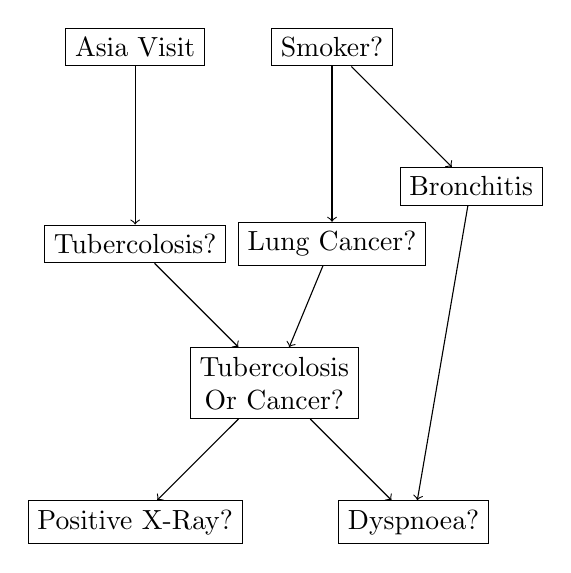
\begin{tikzpicture}[node distance={25mm}, main/.style = {draw, align=center}]
	%% Nodes
	\node[main] (1) {Asia Visit};
	\node[main][right of=1] (2) {Smoker?};

	\node[main][below of=1] (3) {Tubercolosis?};

	\node[main][right of=3] (4) {Lung Cancer?};
	\node[main][below right of=2] (5) {Bronchitis};

	\node[main][below right of=3] (6) {Tubercolosis\\Or Cancer?};          

	\node[main][below left of=6] (7) {Positive X-Ray?};

	\node[main][below right of=6] (8) {Dyspnoea?};     


	%% Edges
	\draw[->] (1) -- (3);
	\draw[->] (2) -- (4);
	\draw[->] (2) -- (5);
	\draw[->] (3) -- (6);     
	\draw[->] (4) -- (6);     
	\draw[->] (6) -- (7);               
	\draw[->] (5) -- (8);
	\draw[->] (6) -- (8);
	\end{tikzpicture}
        \vspace{5mm}
    \caption{Asia Network - Missing Evidence.\\}
  \end{subfigure} \hspace{15mm} 
  \begin{subfigure}[t]{0.4\linewidth} \label{subfig:virtual}
	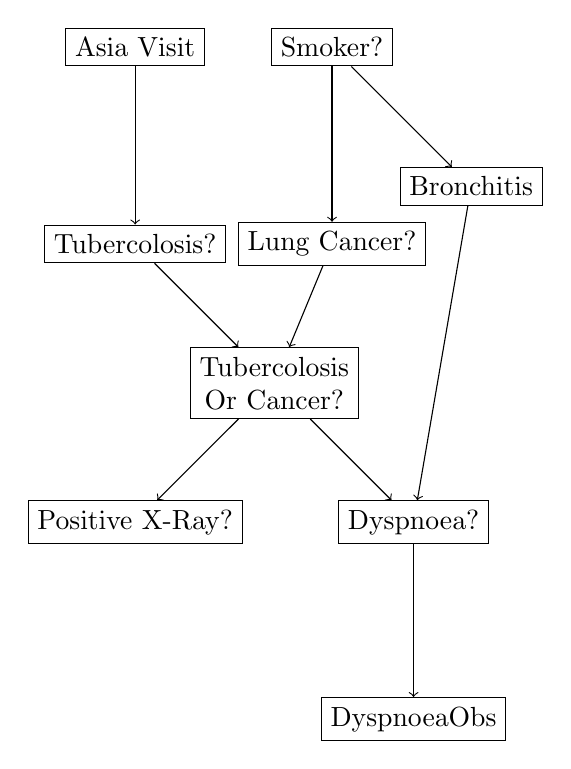
\begin{tikzpicture}[node distance={25mm}, main/.style = {draw, align=center}]
	%% Nodes
	\node[main] (1) {Asia Visit};
	\node[main][right of=1] (2) {Smoker?};

	\node[main][below of=1] (3) {Tubercolosis?};

	\node[main][right of=3] (4) {Lung Cancer?};
	\node[main][below right of=2] (5) {Bronchitis};

	\node[main][below right of=3] (6) {Tubercolosis\\Or Cancer?};          

	\node[main][below left of=6] (7) {Positive X-Ray?};

	\node[main][below right of=6] (8) {Dyspnoea?};     
	\node[draw, distance={10mm}][below of=8] (9) {Dyspnoea \\ Obs};

	%% Edges
	\draw[->] (1) -- (3);
	\draw[->] (2) -- (4);
	\draw[->] (2) -- (5);
	\draw[->] (3) -- (6);     
	\draw[->] (4) -- (6);     
	\draw[->] (6) -- (7);               
	\draw[->] (5) -- (8);
	\draw[->] (6) -- (8);
	\draw[->] (8) -- (9);

	\end{tikzpicture}
        \vspace{5mm}
    \caption{Asia Network - Expanded as by Pearl's Virtual Evidence.}
  \end{subfigure}
  \vspace{0mm}
\end{figure}

Concretely assume as in \cite{Wasserkrug_all} that the NLP correctly
characterizes Dysponea 70\% of the times, when this does in fact
occurs. Note that the NLP tool does not consider any prior
information resulting from the probabilistic structure of our
network. Then you might encode such likelihood evidence of the NLP
as in Table \ref{tb:virt-evidence}.

\begin{table}[!h]

\begin{center}
\begin{tabular}{|l||*{2}{c|}}\hline
\backslashbox{DysponeaObs}{Dysponea?}
&\makebox[3em]{yes}&\makebox[3em]{no}\\\hline\hline
True & 0.7 & 0.3\\\hline
False & 0.3 & 0.7 \\\hline
\end{tabular}
\end{center}

\caption[Virtual Evidence CPT]{DysponeaObs - Virtual Evidence Node CPT}
\label{tb:virt-evidence}
\end{table}

Given such a CPT, encoding the likelihood evidence, it is possible
to set the DyspnoeaObs to true as a hard finding. In such a way you
will work with a standard network that is just composed of missing
and hard evidence. You can then update the cognitive state of your
network by standard inference techniques, and compute the
parameters of interest by a standard EM-algorithm.

Given such explanation it follows that it is possible to rewrite
the EM-step by adjusting the E-step such that it will perform its
inference step on the virtual evidence augmented network that
respects and incorporates the likelihood evidence information. This
was the intuition and contribution of \cite{Wasserkrug_all} and such
an algorithm, with the corresponding modification of the E-step, is
presented in \ref{alg:EM-Likelihood}.

We continue the next section by modifying such algorithm such that
it is possible to perform MAP estimation in Bayesian settings.


\algrenewcommand\algorithmicindent{1.5em}%

\begin{algorithm*}[h!]
\caption{EM-Likelihood: an EM algorithm for learning with likelihood evidence}
\label{alg:EM-Likelihood}
%\begin{\algsize}
\vspace{-10pt}
\begin{multicols}{2}
\begin{algorithmic}[1] 
\Require Bayesian network $\mathcal{B}=\langle \mathbf{X},\mathbf{D}, G, \mathbf{P} \rangle$, dataset $S$ 

\Procedure{EM}{$\mathcal{B}$, $S$}
\State Initialize $\mathcal{B}$'s parameters $\theta \leftarrow \theta^0$
\ForAll{$t=1, \ldots$ until convergence}
  \State $M-step \ as \ in \ Algorithm \ 1$
\EndFor
\EndProcedure
\\
\Function{Compute-ESS}{$\mathcal{B}=(G,\theta)$, $S$} 

\ForAll {$i\in1,\ldots,n$}
  \ForAll {$x_{i},u_{i}\in Val(X_{i},\textbf{PA}_{X_{i}}^{\mathcal{B}})$}
   \State $\bar{M}[x_{i},u_{i}]\leftarrow 0$
  \EndFor
\EndFor

% \State (Go over all evidence nodes, creating an augmented network
% for each one, and collect all of the evidence for the nodes in $G$)
\ForAll{example $S_{j}\in S$}

    \State Let $O_j$ be the observations induced by $S_j$
    \State $(G',\theta') \leftarrow$ \textsc{Augment-BN}($\mathcal{B}=(G,\theta)$, $O_{j}$)
    %  (We'll denote $<G',\theta'>$ by $BN_{i}$ as it is the BN induced by example $i$)
    \ForAll{$o \in O_j$}
      \State Set the value of $o_V$ to $true$
    \EndFor
    \State Run inference on $(G',\theta')$ with evidence $d_{j}$
    \ForAll{i$ = 1,\ldots,n$}
      \ForAll{$x_{i},u_{i}\in Val(X_{i},\textbf{PA}_{X_{i}}^{\mathcal{B}})$}
    
        \State $\bar{M}[x_{i},u_{i}] \mathrel{{+}{=}} P_{(G',\theta')}(x_{i},u_{i}|d_{j})$
    
      \EndFor
    \EndFor
\EndFor
\EndFunction
\\
\Function{Augment-BN}{$\mathcal{B}=(G,\theta)$, $O$} 
  \State Initialize $G'\leftarrow G$, $\theta'\leftarrow\theta$
  \ForAll{$o\in O$}

    \State $G'_{\mathbb{V}}\leftarrow G'_{\mathbb{V}}\cup o_{V}$, $G'_{\mathbb{E}}\leftarrow G'_{\mathbb{E}}\cup(V,o_{V})$      \Comment{Add a new observation node to the graph and connect it to the relevant node}
    \ForAll{$c_{i}\in Conf$}   \Comment{$Conf$ actual likelihood values provided for a node}
      \State $\theta'\leftarrow\theta'\cup\theta_{O_{V}=true|v_{i}}=c_{i}$ \Comment{Set the relevant CPT entry to be $Pr(obs|V=v_{i})$}
    \EndFor
  \EndFor
\State \textbf{return} $(G',\theta')$
\end{algorithmic}
\end{multicols}
%\end{\algsize}
\end{algorithm*}

\newpage

\subsection{Bayesian Learning MAP - Adjusted EM for Likelihood Evidence}
\label{sec:org42b30c7}

The idea of this section is to extend \ref{alg:EM-Likelihood} in
order to obtain the MAP estimator in a Bayesian Learning setting
with Likelihood Evidence.

We discussed in the previous section how likelihood evidence
requires augmenting the core network by virtual evidence nodes as
in \cite{pearl2014probabilistic} and consequently perform the
inference step on such augmented networks.

Such procedure was outlined by the modification of the E-step in
comparison to the standard EM algorithm with missing evidence.

Moreover, we discussed in section \ref{bayes-parameter-learning}, how
it is possible to adjust the M-step of the EM-algorithm to perform
the task of MAP estimation. Both correctness and convergence
properties will apply such that we will converge to a local maximum
for our posterior distribution.

Combining the two steps it is immediate to see that it is possible
to perform Bayesian Parameter Learning under likelihood evidence
by replacing line 4 of \ref{alg:EM-Likelihood} with 

\begin{algorithm*}[h!]
\caption{Replace M-step for Bayesian Parameter Learning}
\label{alg:Bayes-EM-Likelihood}
%\begin{\algsize}
\vspace{-10pt}
\begin{multicols}{2}
\begin{algorithmic}[1] 
\Require Bayesian network $\mathcal{B}=\langle \mathbf{X},\mathbf{D}, G, \mathbf{P} \rangle$, dataset $S$ 

\Function{M-Step}{$\mathcal{B}$, $S$}
   \State $\theta_{x_{i}|u_{i}}^{t+1}=\frac{\bar{M}_{\theta^{t}}[x_{i},u_{i}] + \alpha_i - 1}{\sum_j \bar{M}_{\theta^{t}}[x_{j},u_{i}] + \alpha_j - 1}$\\
   
   \textbf{return} $(\theta^{t+1})$

\end{algorithmic}
\end{multicols}
%\end{\algsize}
\end{algorithm*}

Given such a computation it is possible to get to a local maximum
for the MAP estimator.

\newpage

\section{On Probabilistic Evidence}
\label{probabilistic-em}
In this section we extend the theory presented that far by
introducing some techniques in order to deal with parameter learning
for the case of \emph{non-fixed probabilistic evidence}.

In the previous chapter we showed how it is possible to rephrase a
likelihood evidence as a hard evidence by means of augmenting the
network via \emph{virtual evidence}.

We could then perform the inference step and propagate the
information by means of Bayes Rule updating the probabilistic
structure of the network.

By contrast, with probabilistic evidence such an approach is not
viable. This because, as argued by \cite{PENG_2010}, propagating a
probabilistic finding on \(X_i \in \textbf{X}\) requires a revision of
the probability distribution of the network \(P_\theta(\textbf{X})\)
on \(X_i\) by a local probability distribution defined by the
probabilistic evidence statement \(R(X_i)\). Given that \(R(X_i)\),
although acting as a condition for the update, is not itself an
event, Bayes Rule and standard inference based on message passing
algorithms fail. Hence, as mentioned in \cite{Mrad_2015}, a
probabilistic finding \(R(X_i)\) requires a reconsideration of the
entire joint probability distribution \(P_\theta(\textbf{X})\) because
it replaces the existing \emph{prior} on the variable \(X_i\).

In simple words, in the presence of probabilistic evidence it is not
possible to propagate evidence by standard message passing
algorithms. The solution proposed by \cite{jeffrey1990logic}, is then
to replace the initial probabilistic structure of the network
\(P_\theta(\textbf{X})\) by a new probabilistic structure
\(Q_\theta(\textbf{X})\) that reflects the beliefs in the variables of
the model \emph{after accepting the probabilistic evidence}.

In the specifics, as well outlined by \cite{Mrad_2015}, according to
what is usually referred as Jeffrey's \emph{probability kinematics}, \(Q\)
must satisfy the following requirements:

\begin{enumerate}
\item the posterior probability distribution considering the network
structure on the observed variable \(Q(X_i)\) is unchanged: \(Q(X_i)
     = R(X_i)\). This is in fact the functional requirement of the
probabilistic evidence.

\item the conditional probability distribution of other variables given
\(X_i\) remains invariant under the observation: \(Q(\textbf{X}
     \textbackslash X_i | X_i) = P (\textbf{X} \textbackslash X_i |
     X_i)\). This essentially means that even if P and Q disagree on
\(X_i\), they agree on the consequences of \(X_i\) on other variables
\cite{Mrad_2015}.
\end{enumerate}

With the above specification of a new probabilistic structure
satisfying the functional requirements of probabilistic evidence it
is possible to compute the probability of a given event by means of
Jeffrey's rule:

\begin{equation} \label{eq:Jeffreys_Update}
 Q(\textbf{Z} = z) = \sum_{x_i \in Val(X_i)} P(\textbf{Z} = z | X = x_i) R(X = x_i)
\end{equation}

Albeit being theoretically compelling, Jeffrey's formula above
\ref{eq:Jeffreys_Update}, should not be directly applied in Bayesian
Networks. In fact such a formula requires the specification and
functional form of the full probabilistic structure of the network
in any state of the network in order to compute \(P(\textbf{Z} = z | X_i =
  x_i)\). I.e. in order to compute the new probabilistic structure
Q\textsubscript{\(\theta\)} you would need to perform an inference step over all
possible states combinations. A very computationally intensive task.

The solution to this problem as suggested by \cite{Chan_2005} and
\cite{PENG_2010} is to frame probabilistic evidence into likelihood
evidence by computing the likelihood ratio as defined by:

\begin{align} \label{eq:probabilistic-to-likelihood-evidence}
 L(X_i) = (\frac{R(x_{i_1})}{P(x_{i_1})}: ... : \frac{R(x_{i_k})}{P(x_{i_k})})
\end{align}

It is then possible to prove that propagating such likelihood
evidence by means of Pearl's method as described in the previous
section, is equivalent to propagating and obtaining the probabilistic
structure by means of Jeffrey's method \ref{eq:Jeffreys_Update}.

It is in fact possible to prove, as in \cite{PENG_2010}, that with
such an approach the posterior probability of \(X_i\) after propagating
\(L(X_i)\) by Pearl’s method, is equal to \(R(X_i)\).

Given such theory it is straightforward to understand that
in the case of a single probabilistic evidence we can easily learn
the parameters of the Bayesian Network via the following adjustment
of the \textbf{AUGMENT-BN} function of \ref{alg:EM-Likelihood}

\algrenewcommand\algorithmicindent{1.5em}%

\begin{algorithm*}[h!]
\caption{EM-Single Probabilistic Evidence: an EM algorithm for learning in the case of a single probabilistic evidence}
\label{alg:EM-Probabilistic-Evidence}
%\begin{\algsize}
\vspace{-10pt}
\begin{multicols}{2}
\begin{algorithmic}[1] 
\Require Bayesian network $\mathcal{B}=\langle \mathbf{X},\mathbf{D}, G, \mathbf{P} \rangle$, dataset $S$, Observations $O$

\Function{Augment-BN}{$\mathcal{B}=(G,\theta)$, $O$} 
  \State Initialize $G'\leftarrow G$, $\theta'\leftarrow\theta$, $Conf \leftarrow \emptyset$
  \ForAll{$r_{j_i}\in ProbEv(x_j)$}  \Comment{$ProbEv$ is the passed probabilistic evidence. r are the states for the Node.}
    \State {$Conf \leftarrow Conf \cup \frac{r_{j_i}}{\mathbf{P}_{x_{j_i}}}$}
  \EndFor
  \ForAll{$o\in O$}
    \State $G'_{\mathbb{V}}\leftarrow G'_{\mathbb{V}}\cup o_{V}$, $G'_{\mathbb{E}}\leftarrow G'_{\mathbb{E}}\cup(V,o_{V})$      \Comment{Add a new observation node to the graph and connect it to the relevant node}
    \ForAll{$c_{i}\in Conf$}   \Comment{$Conf$ computed likelihood for a probabilistic node}
      \State $\theta'\leftarrow\theta'\cup\theta_{O_{V}=true|v_{i}}=c_{i}$ \Comment{Set the relevant CPT entry to be $Pr(obs|V=v_{i})$}
    \EndFor
  \EndFor
\State \textbf{return} $(G',\theta')$
\end{algorithmic}
\end{multicols}
%\end{\algsize}
\end{algorithm*}

It is important to mention, to this point that in the case of
multiple probabilistic evidence on different nodes, the above
approach does not apply.

This because, as shown by example in \cite{PENG_2010}, the algorithm
above is not commutative and does not guarantee the functional
requirement \(R(X_i) = Q(X_i)\) for at least one node \(i\). This
intuitively because it just guarantees the functional property for the last
virtual node for which inference is propagated using Pearl virtual
evidence method.

This is for instance what happens in \cite{PENG_2010} with two
probabilistic evidence, \(R(X_1), R(X_2)\) and the property that
\(Q(X_1) \neq R(X_1)\) or \(Q(X_2) \neq R(X_2)\), depending on the
order of propagation.

In order to solve such an issue, and guarantee the functional
requirement of probabilistic evidence, the \emph{Iterative Proportional
Fitting Procedure (IPFP) algorithm} was proposed by
\cite{Valtorta_2002}.

The algorithm is based on the following theorem as reported in
\cite{PENG_2010}:

\begin{theorem}\label{thm:two-I-projection}
Let $Q_i(\textbf{X})$ be the distribution resulting from updating $P(\textbf{X})$ by $R(X_i)$,
$X_i \subset \textbf{X}$ using Jeffrey’s rule described above. Then $Q_i(\textbf{X})$ is the I-projection of $P(\textbf{X})$ on
$\textbf{P}_{R(X_i)}$, where $\textbf{P}_{R(X_i)}$ is the set of distributions whose marginal over $X_i$ equal $R(X_i)$.
\end{theorem}

The idea of the IPFP algorithm is then the one of allowing multiple
probabilistic evidence by leveraging the theorem above.

As well outlined in \cite{PENG_2010}, the idea is in fact to modify
\(P(\textbf{X})\) incorporating the multiple constraints arising from
the multiple probabilistic evidence conditions passed by the
user. Consider \(j = 1, ..., J\) restrictions, then you can perform
such an exercise by iteratively projecting the distribution
resulted from the previous iteration \(\textbf{P}_{R(X_j)}\) on the
next set of constraints \(R(X_{j+1})\).

Formally the IPFP would look as follows:

\algrenewcommand\algorithmicindent{1.5em}%

\begin{algorithm*}[h!]
\caption{IPFP Algorithm}
\label{alg:IPFP-algorithm}
%\begin{\algsize}
\vspace{-10pt}
\begin{multicols}{2}
\begin{algorithmic}[1] 
\Require Probabilistic Evidence $R(X_j, ..., X_J)$, intial distribution $P(\textbf{X})$, necessary condition $R(X_j) << Q_{k-1}(X_j) \ \forall \ k$

\Function{IPFP-Distribution}{$Q_k(\textbf{X})$} 
  \State Initialize $Q_0(\textbf{X}) \leftarrow P(\textbf{X})$
  \For{$k = 1, ..., m = 1 + (k \ {-} \ 1) \ mod \ J$}
    \State {

$Q_k(x) = \left\{
\begin{array}{ll}
Q_{k-1}(x) * \frac{R(x_j)}{Q_{k-1}(x_j)}
& Q_{k-1}(x_j) \geq 0 \\
0 & \, else \\
\end{array}
\right. $} \Comment{note that $j$ represent the constraint used at each iteration }
  \EndFor
\end{algorithmic}
\end{multicols}
%\end{\algsize}
\end{algorithm*}

As proved by several authors such method converge. Moreover, given
the new probabilistic structure \(Q_k(\textbf{X})\) that reflects the
beliefs in the variables of the model \emph{after accepting the
probabilistic evidence}, we can learn the parameters of the network
using the standard EM-algorithm.

It holds in fact that given complete or missing evidence we can
leverage the theory developed in the previous chapters to learn the
parameters of a network displaying multiple probabilistic evidence
by leveraging the updated network probabilistic structure
\(Q_k(\textbf{X})\) at the inference step in the E-step.

This is summarized in algorithm \ref{alg:EM-Probabilistic}.

\algrenewcommand\algorithmicindent{1.5em}%

\begin{algorithm*}[h!]
\caption{EM-Proabilistic: an EM algorithm for learning with probabilistic evidence}
\label{alg:EM-Probabilistic}
%\begin{\algsize}
\vspace{-10pt}
\begin{multicols}{2}
\begin{algorithmic}[1] 
\Require Bayesian network $\mathcal{B}=\langle \mathbf{X},\mathbf{D}, G, \mathbf{P} \rangle$, dataset $S$ 

\Procedure{EM}{$\mathcal{B}$, $S$}
\State Initialize $\mathcal{B}$'s parameters $\theta \leftarrow \theta^0$
\ForAll{$t=1, \ldots$ until convergence}
  \State $M-step \ as \ in \ Algorithm \ 1$
\EndFor
\\
\Function{Compute-ESS}{$\mathcal{B}=(G, \theta)$}

\State {Run IPFP given current parameterization}\Comment {Note - you have to perform such  iteration at each iteration}
\State {$Q \leftarrow$ Return convergence distribution of algorithm IPFP above} 

\ForAll {$i\in1,\ldots,n$}
  \ForAll {$x_{i},u_{i}\in Val(X_{i},\textbf{PA}_{X_{i}}^{\mathcal{B}})$}
   \State $\bar{M}[x_{i},u_{i}]\leftarrow 0$
  \EndFor
\EndFor

\ForAll{example $S_{j}\in S$}

    \State {Run inference on $(G, Q_k, \theta)$ with evidence $d_{j}$}

    \ForAll{i$ = 1,\ldots,n$}
      \ForAll{$x_{i},u_{i}\in Val(X_{i},\textbf{PA}_{X_{i}}^{\mathcal{B}})$}

        \State $\bar{M}[x_{i},u_{i}] \mathrel{{+}{=}} Q_{(G,\theta)}(x_{i},u_{i}|d_{j})$ \Comment {Note that inference is based on the adjusted distriution Q obtained above}
      \EndFor
    \EndFor
\EndFor
\EndProcedure

\end{algorithmic}
\end{multicols}
%\end{\algsize}
\end{algorithm*}

We note two problems, the first being that
the algorithm needs to perform IPFP at each E-step given the new
parameterization. You run in fact a chicken-egg problem that makes
the solution to such problem very expensive. IPFP requires the
parameterization of the node to be known in order to perform
inference and get to the updated probabilistic structure of the
network after consider probabilistic evidence. But we desire to
learn such a parameterization such that we need to repeat the above
until convergence.

Moreover, we note that IPFP requires to run inference and compute the
new probabilistic structure for all possible realizations in the
network \(x \in Val(\textbf{X})\). In order to perform such task the
full joint probability distribution P(\textbf{X}) is be necessary. It
is obvious that for big Bayesian Networks the task of estiamting the
full-joint would be often infeasible to compute without the help of cost
efficient inference algorithms such as the clique tree/ junction tree algorithms.

In this sense, further refinements were propose such as the \emph{big
clique} and the \emph{modified junction tree} as discussed in
\cite{Valtorta_2002}.

Both of such algorithms leverage the ideas of the clique trees
algorithms as proposed by \cite{shafer1990probability}. As well
explained in \cite{koller2009probabilistic}, using clique algorithms
it is possible to run the inference and get the entire joint
P(\textbf{X}) in an efficient way by propagating up- and downstreams
the messages with the factor updates of interest. In such a way it is
possible to get the entire joint-proability of the network in a
computationally efficient way.

However, note that the clique tree inference algorithms as proposed by
\cite{shafer1990probability} are not applicable in the general case of
proabilistic evidence. This because, as mentioned in
\cite{Valtorta_2002}, in the case of probabilistic evidence `after
updating using all evidence, we still require that all appropriate
marginals of the updated distribution be equal to the evidence
entered. The deservedly celebrated junction tree algorithm for
probability update was not designed to satisfy this requirement and in
fact it does not`. A proof of that is provided by example in
\cite{Valtorta_2002} and we refer to it for further details.

In order to deal with that issue in the case of multiple probabilistic evidence,
\cite{Valtorta_2002} proposed two extensions of the classical junction
tree with different benefits in terms of time and space
efficiencies. These are as mentioned the \emph{big clique} and the
\emph{modified junction tree}, which will be briefly discussed next.

Starting with the \emph{modified junction tree}, the idea is to
guarantee the first property of Jeffrey's probability kinematics -
i.e. the property of the unchanged posterior probailistic evdience -
by embedding an IPFP step into the classical junction tree
algorithm. Such IPFP step at propagation time together with the
iteration of the procedure until convergence, will guarantee that the
converged propbability satisfies the two functional requirements of
Jeffrey's probability kinematics as proved in
\cite{csiszar1975divergence}.

Important is, once more, to note the high computational
costs of applying such an algorithm given the necessary IPFP step
embedded at propagation time and the need to repeat the cycle until
convergence as outlined in \cite{Valtorta_2002}. Two iterations cycles are
involved in such an algorithm that would then be embedded in the E-step
cycles of the EM-algorithm necessary for performing the parameter learning task. 

A better solution might be the one of leveraging the \emph{big clique}
algorithm of \cite{Valtorta_2002}. There a single iteration procedure
is involved - i.e. a single IPFP run - at the cost of a less space
efficient procedure involving the creation of a \emph{big clique}
containing all of the specified probabilistic evidences.

Note that both of the techniques proposed by \cite{Valtorta_2002}
build on the theoretical fundamentals of IPFP and junction
trees. However, both involve refactoring the existing junction tree
inference engine to either embed an IPFP cycle into it or by
creating the necessary big-cliques of interest by adding undirected
edges connecting all of the variables involving probabilistic
evidence.

In this sense, two further algorithms were proposed by
\cite{PENG_2010}. These do not impose refactoring of the junction tree
inference process but rather leverage a likelihood evidence
reformulation. These algorithms are then especially useful as they
allow a quick implementation in statistical software such as
\href{https://github.com/radum2275/merlin}{merlin}. The inference step based on junction trees algorithm would
not be altered in this case but a rather simple adjustment takes
place before the inference step by creating a synthetic network
embedding the probabilistic evidence information.

Finally, it is also important to realize that the two algorithms
increases the set of time-space complexity mixtures and may
therefore be the best inference solution depending on the number of
probabilistic evidences as well on the network size of interest.

For the exact algorithmic formula of the two algorithm we refer to
the paper of \cite{PENG_2010}. We note that, as mentioned by the
authors, BN-IPFP-2 updates the joint distribution of the variable
involving probabilistic evidence, while and BN-IPFP-1 updates the
belief of the whole bayesian network such that the trade-offs are
similar in spirit to the one of the standard IPFP and junction-tree
based algorithms.

We conclude by expressing algorithm
\ref{alg:EM-Multiple-Probabilistic} in order to perform parameter
learning in the case of multiple probabilistic evidence R(\textbf{Y}) with
\(\textbf{Y} = {Y_1, ..., Y_J}\) - i.e. a multivariate random
variable composed of \emph{j} probabilistic evidences.

\algrenewcommand\algorithmicindent{1.5em}%

\begin{algorithm*}[h!]
\caption{EM-Proabilistic: an EM algorithm for learning with multiple probabilistic evidence}
\label{alg:EM-Multiple-Probabilistic}
%\begin{\algsize}
\vspace{-10pt}
\begin{multicols}{2}
\begin{algorithmic}[1] 
\Require Bayesian network $\mathcal{B}=\langle \mathbf{X}, \mathbf{Y},\mathbf{D}, G, \mathbf{P} \rangle$, dataset $S$ 

\Procedure{EM}{$\mathcal{B}$, $S$}
\State Initialize $\mathcal{B}$'s parameters $\theta \leftarrow \theta^0$
\ForAll{$t=1, \ldots$ until convergence}
  \State $M-step \ as \ in \ Algorithm \ 1$
\EndFor
\\
\Function{Compute-ESS}{$\mathcal{B}=(G, \theta)$}
\State {$Q \leftarrow$ BN-IPFP-1($\mathcal{B}, R(X_1, ..., X_j, ...,X_J), P(\textbf{X}), S$)} \Comment {You can also alternatively use BN-IPFP-2 as in PENG et. all paper.}

\ForAll {$i\in1,\ldots,n$}
  \ForAll {$x_{i},u_{i}\in Val(X_{i},\textbf{PA}_{X_{i}}^{\mathcal{B}})$}
   \State $\bar{M}[x_{i},u_{i}]\leftarrow 0$
  \EndFor
\EndFor

\ForAll{example $S_{j}\in S$}
    \ForAll{i$ = 1,\ldots,n$} \Comment {Run inference on $(G, Q_k, \theta)$ with evidence $D$ and compute ESS}
      \ForAll{$x_{i},u_{i}\in Val(X_{i},\textbf{PA}_{X_{i}}^{\mathcal{B}})$}

        \State $\bar{M}[x_{i},u_{i}] \mathrel{{+}{=}} Q_{(G,\theta)}(x_{i},u_{i}|d_{j})$ \Comment {Note that inference is based on the adjusted distriution Q obtained above}
      \EndFor
    \EndFor
\EndFor
\EndFunction
\\
\Function{BN-IPFP-1}{$\mathcal{B}, R(X_1, ..., X_j, ...,X_J), P(\textbf{X}), S$}

\State{$Q_0 = P(\textbf{X}), k = 1$}
\\
\While {no convergence in the Q distribution}

  \State $j = 1 + (k-1) \ mod \ m; l = 1 + \floor*{\frac{k-1}{m}}$
  \State $L_{j,l}(Y^j) = \frac{R(y^j_{(1)})}{Q_{k-1}(y^j_{(1)})} : \ldots : \frac{R(y^j_{(j_s)})}{Q_{k-1}(y^j_{(j_s)})}$ \Comment{Construct virtual evidence with likelihood ratio}
  \State {where $y^j_{(1)}, \ldots, y^j_{(j_s)}$ are state configurations of $Y^j$}
\\
  \State {Obtain $Q_{k}$ by updating $Q_{k-1}$ with $L_{j,l}(Y^j)$ using Pearl's virtual evidence method}
\\
  \State {$k \mathrel{{+}{=}} 1$ 

\EndWhile
\EndProcedure

\end{algorithmic}
\end{multicols}
%\end{\algsize}
\end{algorithm*}

\cleardoublepage

\section{Conclusion, Criticalities and Further Work}
\label{conclusion}
In this script we exposed the theoretical background in order
to deal with the parameterization riddle of Bayesian Networks.

The theory was elaborated bottom up. Starting with the most basic
case of \emph{complete evidence} we showed the property of local and
global likelihood decomposition in Bayesian Networks. It was then
straightforward to see that both in the case of Maximum Likelihood
Estimation as well as in the case of Bayesian Learning it was
possible to estimate the parameters by optimizing the individual
CPDs.

Turning to the case of \emph{missing evidence} we showed that the above
properties are lost. Despite this, we formally proved that it is
possible to apply the EM-algorithm in order to reach a local
optimum. Moreover, we argued how after the inference step the global
\emph{expected} likelihood decomposition is satisfied such that it is
possible to maximize the parameters of the individual CPDs
independently in such a step.

We continued by introducing the case of parameter learning under
likelihood evidence as presented in \cite{Wasserkrug_all}. The key
there was to recognize the possibility of extending the bayesian
network by incorporating the likelihood evidence by the means of
virtual evidence nodes as proposed by
\cite{pearl1987evidential}. Given such a method it was possible to
frame likelihood evidence as hard-evidence, such that by the
"elimination" of it, the network evidence would just consists of
missing-evidence and hard-evidence. In that case, the classical
EM-algorithm as discussed in section \ref{missing-learning} applies.

On the top of the arguments proposed by \cite{Wasserkrug_all} we
showed that it is possible to extend the EM-algorithm to the case of
maximum a posterior Bayesian parameter learning without loosing the
correctness and convergence properties of the algorithm. In the
specific we showed that the inference step; i.e. the expectation is
unaltered by the introduction of the priors in Bayesian
Networks. However, the M-step must be adjusted in order to take the
influence of the prior into account. In this sense we extended the
\href{https://github.com/radum2275/merlin}{merlin} engine to deal with case of Bayesian Learning for the case of
Multinomial-Dirichlet CPDs both in the case of missing evidence and
likelihood evidence. Moreover, we exposed the general theory for
generalizing the modeling possibilities to the case of exponential
families CPDs and we exposed the possibility of leveraging
M-projection in order to estimate the parameters of choice in that
case.

Finally, we turned to the case involving probabilistic
evidence. There again the epiphany comes with the realization that
after the specification of a probabilistic network structure taking
the probabilistic evidence constraints into account it is possible
to choose the parameterization maximizing such an adjusted
constrained probabilistic structure via the classical EM-algorithm.
In this sense, the difficulty consists in finding ways to
economically reach the new network probabilistic structure
satisfying the probabilistic evidence constraints. This especially
considering the fact that at each step of the EM algorithm, a new
probabilistic structure for the entire network under the given
parameterization has to be computed. We briefly introduced the IPFP
theorem that poses the theoretical fundamental to obtain the network
probabilistic structure of choice. We then exposed multiple modeling
possibilities to incorporate the IPFP step - or derivate of it -
into the EM algorithm. We mentioned the algorithms of
\cite{Valtorta_2002} offering good performance and different
space-time complexity trade-off. We noted then that implementing such
algorithms in statistical software would require to refactor the
entire code-base of the junction tree algorithm used at inference
step. Moreover, they are restricted by definition to the usage of
junction tree algorithms at inference time. Given the above, we
proposed and partially implemented the algorithms of
\cite{PENG_2010}. These are particularly interesting both for their
characteristic of expanding the time-space complexity trade-off
of the models of \cite{Valtorta_2002} as well due to their
characteristic of working via Pearl's virtual evidence
method. Especially the latter property is useful as it allows both
to quickly implement the algorithm in statistical software, as we
performed in \href{https://github.com/radum2275/merlin}{merlin}, as well as perform the inference step with any
algorithm of choice.

Overall, we therefore extended the theory introduced by
\cite{Wasserkrug_all} by noting that extensions of the EM algorithm
are possible and easily integrable in statistical software as was
demonstrated in \href{https://github.com/radum2275/merlin}{merlin}. We both proposed extension of the algorithm
to deal with maximum a posteriori parameter estimation for the case
of Bayesian Learning as well as extensions dealing with
probabilistic evidence. For both we argued that the theory on which
the EM-algorithm relies is satisfied such that we continue to hold
the correctness and convergence properties of the algorithm.

We conclude by noting that upon the realization that the
EM-algorithm consists of an inference and maximization step given a probabilistic
joint distribution specified by the Bayesian Network it comes as no
surprise that once the probabilistic structure implied by the
network satisfies all of the constrains implied by uncertain
evidence, the EM-algorithm will find a local maxima parameterization
of it. When dealing with uncertain evidence the difficulty consists
therefore much more in computing such constrained joint-probability
in a computational way that is time and space efficient rather than
in a fundamental re-elaboration of the EM-algorithm itself.

\subsection{Criticalities and Further Work}
\label{sec:org3be55b0}

The general flaw with this script, is the fact that it focuses
on the theoretical possibilities of the parameterization learning
task in Bayesian Networks without an in depth analysis of the
computational burden to obtain it. In this sense, a deeper analysis
of the computational effort of applying each algorithm is
necessary. This both at an algebraic level as well as in an
empirical way performing some simulation exercise as in
\cite{Wasserkrug_all}\footnote{Consider in this sense the \href{https://www.hugin.com/}{hugin} engine.}.  

Starting with the case of maximum a posteriori distribution for the
case of Bayesian Learning we discussed the limitation of working
with well known conjugate priors such that the posterior
distribution will be a well known distribution. On the other hand,
we briefly touched on the possibility of relying on simulation
techniques in order to get to the maximum a posteriori
parameterization. Finally, we mentioned the possibility of finding
the maximum of the posteriori distribution via gradient-based
numerical methods. An in depth study of such algorithms and
especially of the performance of \cite{meng2016method} would be of
particular interest. 

Turning to the case of the application of the EM-algorithm in the
case of uncertain evidence, an in depth computational analysis of
the algorithm is especially important. This because it is necessary
to obtain a constrained joint-distribution \emph{Q}, taking the uncertain
evidence into account, \emph{at each step of the EM-algorithm} until
convergence. You therefore see that the costs of obtaining a new
constrained joint-distribution is scaled linearly in the numbers of
necessary iterations steps. Therefore, it is especially important
to find the right combination of time-space computational effort
such that the overall effort of obtaining the constrained
joint-distribution and performing inference in the network is
minimized for the network of interest. In this sense, it might be
useful to elaborate some rule of thumb theory to choose the most
suitable algorithm for different classes of Bayesian
Networks. Finally, due to such especially important issues, it might
be meaningful to further implement the algorithms of
\cite{Valtorta_2002} into statistical software as \href{https://github.com/radum2275/merlin}{merlin} in order to
increase the time-space computational mix available and leverage
the best possible algorithm for each network configuration.

We conclude by noting that due to the vast literature and modeling
possibilities available for Bayesian Networks the presented theory
just scratches the surface of the possible algorithms available for
obtaining the most suitable network parameterization. A further
avenue of research that we completely ignored in the script is
the one of performing the inference step via approximate inference
methods and the inspection of the behaviour of the EM-algorithm
method in such a case. Introductory reading material and relevant
literature may be found in \cite{koller2009probabilistic}. We close
by noting that an analysis of the benefits of combining such methods
in computational involving cases such as in the case of the
algorithms dealing with uncertain evidence might be particularly
interesting.

\newpage

\bibliography{../literature/references}

\bibliographystyle{plainnat}

%%%%%%%%%%%%%%%%%%%%%%%%%%%%%%%%%%%%%%%%%%%%%%%%%%
%%% Declaration of originality (Do not remove!)%%%
%%%%%%%%%%%%%%%%%%%%%%%%%%%%%%%%%%%%%%%%%%%%%%%%%%
%% Instructions:
%% -------------
%% fill in the empty document confirmation-originality.pdf electronically
%% print it out and sign it
%% scan it in again and save the scan in this directory with name
%% confirmation-originality-scan.pdf
%%
%% General info on plagiarism:
%% https://www.ethz.ch/students/en/studies/performance-assessments/plagiarism.html
\cleardoublepage
\includepdf[pages={-}, scale=1]{./pdf/confirmation-originality.pdf}
\end{article}
\end{document}
